% Options for packages loaded elsewhere
\PassOptionsToPackage{unicode}{hyperref}
\PassOptionsToPackage{hyphens}{url}
%
\documentclass[
]{article}
\usepackage{amsmath,amssymb}
\usepackage{lmodern}
\usepackage{iftex}
\ifPDFTeX
  \usepackage[T1]{fontenc}
  \usepackage[utf8]{inputenc}
  \usepackage{textcomp} % provide euro and other symbols
\else % if luatex or xetex
  \usepackage{unicode-math}
  \defaultfontfeatures{Scale=MatchLowercase}
  \defaultfontfeatures[\rmfamily]{Ligatures=TeX,Scale=1}
\fi
% Use upquote if available, for straight quotes in verbatim environments
\IfFileExists{upquote.sty}{\usepackage{upquote}}{}
\IfFileExists{microtype.sty}{% use microtype if available
  \usepackage[]{microtype}
  \UseMicrotypeSet[protrusion]{basicmath} % disable protrusion for tt fonts
}{}
\makeatletter
\@ifundefined{KOMAClassName}{% if non-KOMA class
  \IfFileExists{parskip.sty}{%
    \usepackage{parskip}
  }{% else
    \setlength{\parindent}{0pt}
    \setlength{\parskip}{6pt plus 2pt minus 1pt}}
}{% if KOMA class
  \KOMAoptions{parskip=half}}
\makeatother
\usepackage{xcolor}
\usepackage[margin=1in]{geometry}
\usepackage{longtable,booktabs,array}
\usepackage{calc} % for calculating minipage widths
% Correct order of tables after \paragraph or \subparagraph
\usepackage{etoolbox}
\makeatletter
\patchcmd\longtable{\par}{\if@noskipsec\mbox{}\fi\par}{}{}
\makeatother
% Allow footnotes in longtable head/foot
\IfFileExists{footnotehyper.sty}{\usepackage{footnotehyper}}{\usepackage{footnote}}
\makesavenoteenv{longtable}
\usepackage{graphicx}
\makeatletter
\def\maxwidth{\ifdim\Gin@nat@width>\linewidth\linewidth\else\Gin@nat@width\fi}
\def\maxheight{\ifdim\Gin@nat@height>\textheight\textheight\else\Gin@nat@height\fi}
\makeatother
% Scale images if necessary, so that they will not overflow the page
% margins by default, and it is still possible to overwrite the defaults
% using explicit options in \includegraphics[width, height, ...]{}
\setkeys{Gin}{width=\maxwidth,height=\maxheight,keepaspectratio}
% Set default figure placement to htbp
\makeatletter
\def\fps@figure{htbp}
\makeatother
\setlength{\emergencystretch}{3em} % prevent overfull lines
\providecommand{\tightlist}{%
  \setlength{\itemsep}{0pt}\setlength{\parskip}{0pt}}
\setcounter{secnumdepth}{-\maxdimen} % remove section numbering
\ifLuaTeX
  \usepackage{selnolig}  % disable illegal ligatures
\fi
\IfFileExists{bookmark.sty}{\usepackage{bookmark}}{\usepackage{hyperref}}
\IfFileExists{xurl.sty}{\usepackage{xurl}}{} % add URL line breaks if available
\urlstyle{same} % disable monospaced font for URLs
\hypersetup{
  pdftitle={Pancreatic Fat Analysis},
  pdfauthor={Cameron Severn \& Laura Pyle},
  hidelinks,
  pdfcreator={LaTeX via pandoc}}

\title{Pancreatic Fat Analysis}
\author{Cameron Severn \& Laura Pyle}
\date{14 November, 2022}

\begin{document}
\maketitle

{
\setcounter{tocdepth}{2}
\tableofcontents
}
\hypertarget{summary}{%
\section{Summary}\label{summary}}

The following models explore the effect of puberty and Obesity on a
pancreatic fat. Mixed effects models were used with a random intercept
by patient yielding a model which effectively controls for baseline
values of each measure and estimates the change experienced by a patient
by Tanner 5.

Example Interpretation: Liver Fat Percentage

Figure: Raw data (points) plotted with model estimated means with error
bars representing 95\% Confidence Intervals.

Table 1: T-table

(Intercept) - The estimated mean liver fat percentage for a normal
weight patient at Tanner 2/3 is 1.339 (NS)

study\_visit\_number\_svlTanner 5 - The difference between Tanner 2/3
and Tanner 5 is 0.869 for a normal weight patient (NS)

study\_phaseObese - The difference between a normal weight and obese
patient at Tanner 2/3 is 6.292 (p = 0.003)

study\_visit\_number\_svlTanner 5:study\_phaseObese - The difference in
delta liver fat between normal weight and obese patients is -0.599 (More
negative or less positive) (NS). Simple interpretation: Difference in
slope or trajectory.

Table 2: Model Means

This one should be pretty self-explanatory. Group Means as estimated by
the model.

Table 3: Contrasts by Group

Using the same model, contrast statements are used to test differences
in means between discrete groups of patients. Here we see differences
between Obese and Normal Weight patients at each Tanner Stage

Table 4: Contrasts by Tanner Stage

Similar to table 3, but looking at differences between Tanner 5 and
Tanner 2/3 by Obesity Group.

\begin{longtable}[]{@{}
  >{\raggedright\arraybackslash}p{(\columnwidth - 10\tabcolsep) * \real{0.1825}}
  >{\raggedright\arraybackslash}p{(\columnwidth - 10\tabcolsep) * \real{0.2698}}
  >{\centering\arraybackslash}p{(\columnwidth - 10\tabcolsep) * \real{0.1746}}
  >{\centering\arraybackslash}p{(\columnwidth - 10\tabcolsep) * \real{0.1508}}
  >{\centering\arraybackslash}p{(\columnwidth - 10\tabcolsep) * \real{0.1508}}
  >{\centering\arraybackslash}p{(\columnwidth - 10\tabcolsep) * \real{0.0714}}@{}}
\toprule()
\begin{minipage}[b]{\linewidth}\raggedright
study\_visit\_number\_svl
\end{minipage} & \begin{minipage}[b]{\linewidth}\raggedright
\end{minipage} & \begin{minipage}[b]{\linewidth}\centering
Normal Weight (N=24)
\end{minipage} & \begin{minipage}[b]{\linewidth}\centering
Obese (N=16)
\end{minipage} & \begin{minipage}[b]{\linewidth}\centering
Total (N=40)
\end{minipage} & \begin{minipage}[b]{\linewidth}\centering
p value
\end{minipage} \\
\midrule()
\endhead
Tanner 2/3 & \textbf{Age (years)} & & & & 0.248 \\
& ~~~N & 12 & 10 & 22 & \\
& ~~~Mean (SD) & 11.858 (1.460) & 11.126 (1.405) & 11.525 (1.450) & \\
& ~~~Range & 9.495 - 13.886 & 9.506 - 14.234 & 9.495 - 14.234 & \\
& \textbf{sex\_exam} & & & & 0.029 \\
& ~~~Female & 4 (33.3\%) & 8 (80.0\%) & 12 (54.5\%) & \\
& ~~~Male & 8 (66.7\%) & 2 (20.0\%) & 10 (45.5\%) & \\
& \textbf{race\_eth} & & & & \\
& ~~~Hispanic & 0 (0.0\%) & 7 (70.0\%) & 7 (31.8\%) & \\
& ~~~NHW & 7 (58.3\%) & 0 (0.0\%) & 7 (31.8\%) & \\
& ~~~Black & 1 (8.3\%) & 2 (20.0\%) & 3 (13.6\%) & \\
& ~~~Asian & 3 (25.0\%) & 0 (0.0\%) & 3 (13.6\%) & \\
& ~~~Other & 1 (8.3\%) & 1 (10.0\%) & 2 (9.1\%) & \\
& ~~~Native American & 0 (0.0\%) & 0 (0.0\%) & 0 (0.0\%) & \\
& \textbf{bmi\_z} & & & & \textless{} 0.001 \\
& ~~~N & 12 & 10 & 22 & \\
& ~~~Mean (SD) & 0.029 (0.839) & 3.185 (0.676) & 1.464 (1.775) & \\
& ~~~Range & -1.650 - 0.920 & 2.080 - 4.220 & -1.650 - 4.220 & \\
& \textbf{BMI} & & & & \textless{} 0.001 \\
& ~~~N & 12 & 10 & 22 & \\
& ~~~Mean (SD) & 17.750 (1.901) & 30.970 (4.188) & 23.759 (7.403) & \\
& ~~~Range & 14.900 - 20.800 & 23.000 - 36.300 & 14.900 - 36.300 & \\
& \textbf{BMI Percentile} & & & & \textless{} 0.001 \\
& ~~~N & 12 & 10 & 22 & \\
& ~~~Mean (SD) & 46.800 (25.825) & 98.498 (1.674) & 70.299 (32.322) & \\
& ~~~Range & 4.600 - 76.900 & 94.030 - 99.610 & 4.600 - 99.610 & \\
& \textbf{Waist Circumference Average} & & & & \textless{} 0.001 \\
& ~~~N & 12 & 10 & 22 & \\
& ~~~Mean (SD) & 63.422 (4.860) & 96.906 (8.522) & 78.642 (18.295) & \\
& ~~~Range & 54.600 - 70.600 & 84.900 - 108.500 & 54.600 - 108.500 & \\
& \textbf{Total Cholesterol} & & & & 0.534 \\
& ~~~N & 12 & 10 & 22 & \\
& ~~~Mean (SD) & 138.167 (16.672) & 142.600 (15.981) & 140.182 (16.129)
& \\
& ~~~Range & 113.000 - 175.000 & 120.000 - 167.000 & 113.000 - 175.000
& \\
& \textbf{Triglycerides} & & & & 0.066 \\
& ~~~N & 12 & 10 & 22 & \\
& ~~~Mean (SD) & 88.833 (39.742) & 134.900 (69.893) & 109.773 (58.924)
& \\
& ~~~Range & 49.000 - 169.000 & 65.000 - 272.000 & 49.000 - 272.000 & \\
& \textbf{LDL} & & & & 0.409 \\
& ~~~N & 12 & 10 & 22 & \\
& ~~~Mean (SD) & 81.083 (23.720) & 88.700 (17.289) & 84.545 (20.926)
& \\
& ~~~Range & 57.000 - 145.000 & 65.000 - 125.000 & 57.000 - 145.000 & \\
& \textbf{HDL} & & & & \textless{} 0.001 \\
& ~~~N & 12 & 10 & 22 & \\
& ~~~Mean (SD) & 49.500 (7.477) & 35.700 (7.394) & 43.227 (10.109) & \\
& ~~~Range & 38.000 - 62.000 & 26.000 - 49.000 & 26.000 - 62.000 & \\
& \textbf{Adiponectin} & & & & 0.374 \\
& ~~~N & 12 & 10 & 22 & \\
& ~~~Mean (SD) & 11.367 (4.043) & 9.430 (5.922) & 10.486 (4.956) & \\
& ~~~Range & 6.400 - 18.900 & 3.500 - 22.200 & 3.500 - 22.200 & \\
& \textbf{crp\_lv} & & & & 0.011 \\
& ~~~N & 12 & 9 & 21 & \\
& ~~~Mean (SD) & 0.370 (0.610) & 2.053 (1.960) & 1.091 (1.572) & \\
& ~~~Range & 0.010 - 1.810 & 0.150 - 6.130 & 0.010 - 6.130 & \\
& \textbf{0 minute glucose} & & & & 0.696 \\
& ~~~N & 12 & 10 & 22 & \\
& ~~~Mean (SD) & 84.167 (4.529) & 85.100 (6.488) & 84.591 (5.387) & \\
& ~~~Range & 75.000 - 94.000 & 72.000 - 96.000 & 72.000 - 96.000 & \\
& \textbf{0 minute insulin} & & & & \textless{} 0.001 \\
& ~~~N & 12 & 10 & 22 & \\
& ~~~Mean (SD) & 9.417 (4.889) & 23.700 (9.238) & 15.909 (10.104) & \\
& ~~~Range & 4.000 - 22.000 & 9.000 - 39.000 & 4.000 - 39.000 & \\
& \textbf{Insulin Sensitivity (Si)} & & & & 0.006 \\
& ~~~N & 12 & 10 & 22 & \\
& ~~~Mean (SD) & 10.829 (8.945) & 2.013 (0.748) & 6.822 (7.895) & \\
& ~~~Range & 2.498 - 31.333 & 0.699 - 3.399 & 0.699 - 31.333 & \\
& \textbf{HbA1c} & & & & 0.156 \\
& ~~~N & 12 & 10 & 22 & \\
& ~~~Mean (SD) & 5.192 (0.219) & 5.430 (0.508) & 5.300 (0.388) & \\
& ~~~Range & 4.800 - 5.600 & 4.900 - 6.200 & 4.800 - 6.200 & \\
& \textbf{lept} & & & & \textless{} 0.001 \\
& ~~~N & 12 & 10 & 22 & \\
& ~~~Mean (SD) & 4.175 (5.073) & 32.020 (14.286) & 16.832 (17.388) & \\
& ~~~Range & 0.700 - 19.400 & 12.500 - 55.800 & 0.700 - 55.800 & \\
& \textbf{Leptin:Adiponectin Ratio} & & & & \textless{} 0.001 \\
& ~~~N & 12 & 10 & 22 & \\
& ~~~Mean (SD) & 0.403 (0.538) & 4.073 (2.264) & 2.071 (2.418) & \\
& ~~~Range & 0.069 - 2.064 & 1.761 - 8.514 & 0.069 - 8.514 & \\
& \textbf{pancreatic\_fat\_AVG} & & & & 0.147 \\
& ~~~N & 12 & 10 & 22 & \\
& ~~~Mean (SD) & 1.357 (1.011) & 2.244 (1.710) & 1.760 (1.412) & \\
& ~~~Range & 0.000 - 3.050 & 0.000 - 5.190 & 0.000 - 5.190 & \\
& \textbf{Percent Subq Fat} & & & & \textless{} 0.001 \\
& ~~~N & 11 & 6 & 17 & \\
& ~~~Mean (SD) & 18.910 (9.245) & 53.869 (6.065) & 31.248 (19.012) & \\
& ~~~Range & 10.550 - 40.548 & 42.192 - 59.294 & 10.550 - 59.294 & \\
& \textbf{Percent Visceral Fat} & & & & 0.020 \\
& ~~~N & 11 & 6 & 17 & \\
& ~~~Mean (SD) & 7.647 (3.702) & 12.007 (2.263) & 9.186 (3.845) & \\
& ~~~Range & 3.675 - 15.229 & 8.622 - 15.605 & 3.675 - 15.605 & \\
& \textbf{\% Fat} & & & & \textless{} 0.001 \\
& ~~~N & 12 & 9 & 21 & \\
& ~~~Mean (SD) & 24.733 (6.057) & 44.500 (2.483) & 33.205 (11.096) & \\
& ~~~Range & 16.800 - 36.700 & 41.000 - 47.600 & 16.800 - 47.600 & \\
& \textbf{AST} & & & & 0.899 \\
& ~~~N & 12 & 10 & 22 & \\
& ~~~Mean (SD) & 47.750 (14.284) & 46.800 (20.433) & 47.318 (16.913)
& \\
& ~~~Range & 29.000 - 84.000 & 26.000 - 83.000 & 26.000 - 84.000 & \\
& \textbf{alt} & & & & 0.047 \\
& ~~~N & 12 & 10 & 22 & \\
& ~~~Mean (SD) & 32.417 (4.122) & 49.700 (28.048) & 40.273 (20.582) & \\
& ~~~Range & 28.000 - 42.000 & 27.000 - 108.000 & 27.000 - 108.000 & \\
Tanner 5 & \textbf{Age (years)} & & & & 0.460 \\
& ~~~N & 12 & 6 & 18 & \\
& ~~~Mean (SD) & 13.929 (1.358) & 13.452 (1.011) & 13.770 (1.244) & \\
& ~~~Range & 11.691 - 15.537 & 12.074 - 14.505 & 11.691 - 15.537 & \\
& \textbf{sex\_exam} & & & & 0.317 \\
& ~~~Female & 5 (41.7\%) & 4 (66.7\%) & 9 (50.0\%) & \\
& ~~~Male & 7 (58.3\%) & 2 (33.3\%) & 9 (50.0\%) & \\
& \textbf{race\_eth} & & & & \\
& ~~~Hispanic & 1 (8.3\%) & 5 (83.3\%) & 6 (33.3\%) & \\
& ~~~NHW & 6 (50.0\%) & 0 (0.0\%) & 6 (33.3\%) & \\
& ~~~Black & 1 (8.3\%) & 0 (0.0\%) & 1 (5.6\%) & \\
& ~~~Asian & 3 (25.0\%) & 0 (0.0\%) & 3 (16.7\%) & \\
& ~~~Other & 1 (8.3\%) & 1 (16.7\%) & 2 (11.1\%) & \\
& ~~~Native American & 0 (0.0\%) & 0 (0.0\%) & 0 (0.0\%) & \\
& \textbf{bmi\_z} & & & & \textless{} 0.001 \\
& ~~~N & 12 & 6 & 18 & \\
& ~~~Mean (SD) & 0.276 (0.893) & 3.232 (0.820) & 1.261 (1.664) & \\
& ~~~Range & -1.690 - 1.260 & 2.240 - 4.410 & -1.690 - 4.410 & \\
& \textbf{BMI} & & & & \textless{} 0.001 \\
& ~~~N & 12 & 6 & 18 & \\
& ~~~Mean (SD) & 20.150 (1.994) & 34.917 (6.291) & 25.072 (8.094) & \\
& ~~~Range & 16.800 - 23.500 & 27.000 - 42.500 & 16.800 - 42.500 & \\
& \textbf{BMI Percentile} & & & & 0.002 \\
& ~~~N & 12 & 6 & 18 & \\
& ~~~Mean (SD) & 58.621 (26.547) & 98.522 (1.414) & 71.921 (28.831) & \\
& ~~~Range & 4.560 - 85.930 & 96.590 - 99.710 & 4.560 - 99.710 & \\
& \textbf{Waist Circumference Average} & & & & \textless{} 0.001 \\
& ~~~N & 12 & 6 & 18 & \\
& ~~~Mean (SD) & 73.375 (5.801) & 109.100 (12.014) & 85.283 (19.093)
& \\
& ~~~Range & 65.100 - 81.300 & 92.000 - 127.500 & 65.100 - 127.500 & \\
& \textbf{Total Cholesterol} & & & & 0.481 \\
& ~~~N & 12 & 6 & 18 & \\
& ~~~Mean (SD) & 135.167 (22.490) & 143.333 (23.001) & 137.889 (22.329)
& \\
& ~~~Range & 90.000 - 160.000 & 121.000 - 185.000 & 90.000 - 185.000
& \\
& \textbf{Triglycerides} & & & & 0.075 \\
& ~~~N & 12 & 6 & 18 & \\
& ~~~Mean (SD) & 105.500 (39.830) & 146.000 (47.783) & 119.000 (45.651)
& \\
& ~~~Range & 43.000 - 178.000 & 69.000 - 189.000 & 43.000 - 189.000 & \\
& \textbf{LDL} & & & & 0.319 \\
& ~~~N & 12 & 6 & 18 & \\
& ~~~Mean (SD) & 77.417 (20.161) & 86.667 (11.944) & 80.500 (18.030)
& \\
& ~~~Range & 44.000 - 115.000 & 73.000 - 100.000 & 44.000 - 115.000 & \\
& \textbf{HDL} & & & & 0.235 \\
& ~~~N & 12 & 6 & 18 & \\
& ~~~Mean (SD) & 46.000 (8.739) & 40.500 (9.268) & 44.167 (9.044) & \\
& ~~~Range & 35.000 - 62.000 & 29.000 - 54.000 & 29.000 - 62.000 & \\
& \textbf{Adiponectin} & & & & 0.123 \\
& ~~~N & 12 & 6 & 18 & \\
& ~~~Mean (SD) & 9.892 (3.564) & 7.317 (1.995) & 9.033 (3.309) & \\
& ~~~Range & 4.400 - 15.300 & 5.600 - 11.200 & 4.400 - 15.300 & \\
& \textbf{crp\_lv} & & & & 0.103 \\
& ~~~N & 12 & 6 & 18 & \\
& ~~~Mean (SD) & 0.628 (1.480) & 2.302 (2.681) & 1.186 (2.047) & \\
& ~~~Range & 0.040 - 5.290 & 0.340 - 7.650 & 0.040 - 7.650 & \\
& \textbf{0 minute glucose} & & & & 0.007 \\
& ~~~N & 12 & 6 & 18 & \\
& ~~~Mean (SD) & 80.333 (8.316) & 92.333 (6.186) & 84.333 (9.481) & \\
& ~~~Range & 57.000 - 90.000 & 86.000 - 103.000 & 57.000 - 103.000 & \\
& \textbf{0 minute insulin} & & & & \textless{} 0.001 \\
& ~~~N & 12 & 6 & 18 & \\
& ~~~Mean (SD) & 12.083 (7.645) & 33.500 (11.640) & 19.222 (13.623) & \\
& ~~~Range & 2.000 - 32.000 & 16.000 - 47.000 & 2.000 - 47.000 & \\
& \textbf{Insulin Sensitivity (Si)} & & & & 0.053 \\
& ~~~N & 12 & 6 & 18 & \\
& ~~~Mean (SD) & 4.726 (3.049) & 1.902 (1.729) & 3.785 (2.961) & \\
& ~~~Range & 1.621 - 10.222 & 0.050 - 4.980 & 0.050 - 10.222 & \\
& \textbf{HbA1c} & & & & 0.042 \\
& ~~~N & 12 & 6 & 18 & \\
& ~~~Mean (SD) & 5.342 (0.320) & 5.717 (0.376) & 5.467 (0.376) & \\
& ~~~Range & 4.800 - 5.800 & 5.200 - 6.300 & 4.800 - 6.300 & \\
& \textbf{lept} & & & & \textless{} 0.001 \\
& ~~~N & 12 & 6 & 18 & \\
& ~~~Mean (SD) & 7.283 (6.609) & 50.850 (23.141) & 21.806 (25.147) & \\
& ~~~Range & 0.700 - 18.100 & 15.400 - 76.400 & 0.700 - 76.400 & \\
& \textbf{Leptin:Adiponectin Ratio} & & & & \textless{} 0.001 \\
& ~~~N & 12 & 6 & 18 & \\
& ~~~Mean (SD) & 0.884 (1.000) & 7.558 (3.582) & 3.109 (3.860) & \\
& ~~~Range & 0.053 - 3.291 & 1.375 - 10.631 & 0.053 - 10.631 & \\
& \textbf{pancreatic\_fat\_AVG} & & & & 0.056 \\
& ~~~N & 12 & 6 & 18 & \\
& ~~~Mean (SD) & 1.212 (0.910) & 2.442 (1.650) & 1.622 (1.301) & \\
& ~~~Range & 0.000 - 2.990 & 0.140 - 4.480 & 0.000 - 4.480 & \\
& \textbf{Percent Subq Fat} & & & & \textless{} 0.001 \\
& ~~~N & 12 & 6 & 18 & \\
& ~~~Mean (SD) & 24.261 (14.338) & 53.894 (4.866) & 34.139 (18.617) & \\
& ~~~Range & 9.211 - 46.559 & 47.937 - 58.859 & 9.211 - 58.859 & \\
& \textbf{Percent Visceral Fat} & & & & \textless{} 0.001 \\
& ~~~N & 12 & 6 & 18 & \\
& ~~~Mean (SD) & 6.322 (2.676) & 12.236 (1.564) & 8.294 (3.686) & \\
& ~~~Range & 3.353 - 12.581 & 9.489 - 14.273 & 3.353 - 14.273 & \\
& \textbf{\% Fat} & & & & \textless{} 0.001 \\
& ~~~N & 12 & 5 & 17 & \\
& ~~~Mean (SD) & 24.817 (8.384) & 43.320 (5.031) & 30.259 (11.409) & \\
& ~~~Range & 13.800 - 37.600 & 35.500 - 48.800 & 13.800 - 48.800 & \\
& \textbf{AST} & & & & 0.676 \\
& ~~~N & 12 & 6 & 18 & \\
& ~~~Mean (SD) & 36.500 (16.178) & 33.500 (7.635) & 35.500 (13.734) & \\
& ~~~Range & 25.000 - 85.000 & 28.000 - 48.000 & 25.000 - 85.000 & \\
& \textbf{alt} & & & & 0.004 \\
& ~~~N & 12 & 6 & 18 & \\
& ~~~Mean (SD) & 23.500 (7.255) & 42.167 (16.425) & 29.722 (13.978) & \\
& ~~~Range & 15.000 - 41.000 & 27.000 - 74.000 & 15.000 - 74.000 & \\
\bottomrule()
\end{longtable}

\hypertarget{mixed-models}{%
\section{Mixed Models}\label{mixed-models}}

\newpage

\hypertarget{pancreatic_fat_avg}{%
\subsection{pancreatic\_fat\_AVG}\label{pancreatic_fat_avg}}

\includegraphics{fat_analysis_pancreatic_fat_files/figure-latex/unnamed-chunk-4-1.pdf}

\begin{longtable}[]{@{}
  >{\raggedright\arraybackslash}p{(\columnwidth - 10\tabcolsep) * \real{0.5333}}
  >{\raggedright\arraybackslash}p{(\columnwidth - 10\tabcolsep) * \real{0.1889}}
  >{\raggedright\arraybackslash}p{(\columnwidth - 10\tabcolsep) * \real{0.0667}}
  >{\raggedright\arraybackslash}p{(\columnwidth - 10\tabcolsep) * \real{0.0333}}
  >{\raggedright\arraybackslash}p{(\columnwidth - 10\tabcolsep) * \real{0.0889}}
  >{\raggedright\arraybackslash}p{(\columnwidth - 10\tabcolsep) * \real{0.0889}}@{}}
\caption{T-Table}\tabularnewline
\toprule()
\begin{minipage}[b]{\linewidth}\raggedright
\end{minipage} & \begin{minipage}[b]{\linewidth}\raggedright
Estimated Effect
\end{minipage} & \begin{minipage}[b]{\linewidth}\raggedright
SE
\end{minipage} & \begin{minipage}[b]{\linewidth}\raggedright
DF
\end{minipage} & \begin{minipage}[b]{\linewidth}\raggedright
t-value
\end{minipage} & \begin{minipage}[b]{\linewidth}\raggedright
p-value
\end{minipage} \\
\midrule()
\endfirsthead
\toprule()
\begin{minipage}[b]{\linewidth}\raggedright
\end{minipage} & \begin{minipage}[b]{\linewidth}\raggedright
Estimated Effect
\end{minipage} & \begin{minipage}[b]{\linewidth}\raggedright
SE
\end{minipage} & \begin{minipage}[b]{\linewidth}\raggedright
DF
\end{minipage} & \begin{minipage}[b]{\linewidth}\raggedright
t-value
\end{minipage} & \begin{minipage}[b]{\linewidth}\raggedright
p-value
\end{minipage} \\
\midrule()
\endhead
(Intercept) & 1.359 & 0.373 & 22 & 3.640 & 0.00145 \\
study\_visit\_number\_svlTanner 5 & -0.115 & 0.430 & 14 & -0.268 &
0.79280 \\
study\_phaseObese & 0.810 & 0.553 & 22 & 1.464 & 0.15738 \\
study\_visit\_number\_svlTanner 5:study\_phaseObese & 0.152 & 0.717 & 14
& 0.212 & 0.83552 \\
\bottomrule()
\end{longtable}

\begin{longtable}[]{@{}
  >{\raggedright\arraybackslash}p{(\columnwidth - 12\tabcolsep) * \real{0.2090}}
  >{\raggedright\arraybackslash}p{(\columnwidth - 12\tabcolsep) * \real{0.1940}}
  >{\raggedright\arraybackslash}p{(\columnwidth - 12\tabcolsep) * \real{0.0746}}
  >{\raggedright\arraybackslash}p{(\columnwidth - 12\tabcolsep) * \real{0.0896}}
  >{\raggedright\arraybackslash}p{(\columnwidth - 12\tabcolsep) * \real{0.0448}}
  >{\raggedright\arraybackslash}p{(\columnwidth - 12\tabcolsep) * \real{0.1940}}
  >{\raggedright\arraybackslash}p{(\columnwidth - 12\tabcolsep) * \real{0.1940}}@{}}
\caption{Model Means}\tabularnewline
\toprule()
\begin{minipage}[b]{\linewidth}\raggedright
Group
\end{minipage} & \begin{minipage}[b]{\linewidth}\raggedright
Tanner Stage
\end{minipage} & \begin{minipage}[b]{\linewidth}\raggedright
Mean
\end{minipage} & \begin{minipage}[b]{\linewidth}\raggedright
SE
\end{minipage} & \begin{minipage}[b]{\linewidth}\raggedright
DF
\end{minipage} & \begin{minipage}[b]{\linewidth}\raggedright
95\% CI lower
\end{minipage} & \begin{minipage}[b]{\linewidth}\raggedright
95\% CI upper
\end{minipage} \\
\midrule()
\endfirsthead
\toprule()
\begin{minipage}[b]{\linewidth}\raggedright
Group
\end{minipage} & \begin{minipage}[b]{\linewidth}\raggedright
Tanner Stage
\end{minipage} & \begin{minipage}[b]{\linewidth}\raggedright
Mean
\end{minipage} & \begin{minipage}[b]{\linewidth}\raggedright
SE
\end{minipage} & \begin{minipage}[b]{\linewidth}\raggedright
DF
\end{minipage} & \begin{minipage}[b]{\linewidth}\raggedright
95\% CI lower
\end{minipage} & \begin{minipage}[b]{\linewidth}\raggedright
95\% CI upper
\end{minipage} \\
\midrule()
\endhead
Normal Weight & Tanner 2/3 & 1.36 & 0.373 & 23 & 0.586 & 2.13 \\
Obese & Tanner 2/3 & 2.17 & 0.409 & 22 & 1.321 & 3.02 \\
Normal Weight & Tanner 5 & 1.24 & 0.373 & 14 & 0.443 & 2.04 \\
Obese & Tanner 5 & 2.21 & 0.516 & 14 & 1.100 & 3.31 \\
\bottomrule()
\end{longtable}

\newpage

\begin{longtable}[]{@{}
  >{\raggedright\arraybackslash}p{(\columnwidth - 12\tabcolsep) * \real{0.2716}}
  >{\raggedright\arraybackslash}p{(\columnwidth - 12\tabcolsep) * \real{0.1605}}
  >{\raggedright\arraybackslash}p{(\columnwidth - 12\tabcolsep) * \real{0.2593}}
  >{\raggedright\arraybackslash}p{(\columnwidth - 12\tabcolsep) * \real{0.0741}}
  >{\raggedright\arraybackslash}p{(\columnwidth - 12\tabcolsep) * \real{0.0370}}
  >{\raggedright\arraybackslash}p{(\columnwidth - 12\tabcolsep) * \real{0.0988}}
  >{\raggedright\arraybackslash}p{(\columnwidth - 12\tabcolsep) * \real{0.0988}}@{}}
\caption{Contrasts by Group}\tabularnewline
\toprule()
\begin{minipage}[b]{\linewidth}\raggedright
Test
\end{minipage} & \begin{minipage}[b]{\linewidth}\raggedright
Tanner Stage
\end{minipage} & \begin{minipage}[b]{\linewidth}\raggedright
Estimated Difference
\end{minipage} & \begin{minipage}[b]{\linewidth}\raggedright
SE
\end{minipage} & \begin{minipage}[b]{\linewidth}\raggedright
DF
\end{minipage} & \begin{minipage}[b]{\linewidth}\raggedright
t-ratio
\end{minipage} & \begin{minipage}[b]{\linewidth}\raggedright
p-value
\end{minipage} \\
\midrule()
\endfirsthead
\toprule()
\begin{minipage}[b]{\linewidth}\raggedright
Test
\end{minipage} & \begin{minipage}[b]{\linewidth}\raggedright
Tanner Stage
\end{minipage} & \begin{minipage}[b]{\linewidth}\raggedright
Estimated Difference
\end{minipage} & \begin{minipage}[b]{\linewidth}\raggedright
SE
\end{minipage} & \begin{minipage}[b]{\linewidth}\raggedright
DF
\end{minipage} & \begin{minipage}[b]{\linewidth}\raggedright
t-ratio
\end{minipage} & \begin{minipage}[b]{\linewidth}\raggedright
p-value
\end{minipage} \\
\midrule()
\endhead
Obese - Normal Weight & Tanner 2/3 & 0.810 & 0.553 & 22 & 1.46 &
0.157 \\
Obese - Normal Weight & Tanner 5 & 0.962 & 0.636 & 14 & 1.51 & 0.153 \\
\bottomrule()
\end{longtable}

\begin{longtable}[]{@{}
  >{\raggedright\arraybackslash}p{(\columnwidth - 12\tabcolsep) * \real{0.2857}}
  >{\raggedright\arraybackslash}p{(\columnwidth - 12\tabcolsep) * \real{0.1667}}
  >{\raggedright\arraybackslash}p{(\columnwidth - 12\tabcolsep) * \real{0.2500}}
  >{\raggedright\arraybackslash}p{(\columnwidth - 12\tabcolsep) * \real{0.0714}}
  >{\raggedright\arraybackslash}p{(\columnwidth - 12\tabcolsep) * \real{0.0357}}
  >{\raggedright\arraybackslash}p{(\columnwidth - 12\tabcolsep) * \real{0.0952}}
  >{\raggedright\arraybackslash}p{(\columnwidth - 12\tabcolsep) * \real{0.0952}}@{}}
\caption{Contrasts by Tanner Stage}\tabularnewline
\toprule()
\begin{minipage}[b]{\linewidth}\raggedright
Test
\end{minipage} & \begin{minipage}[b]{\linewidth}\raggedright
Group
\end{minipage} & \begin{minipage}[b]{\linewidth}\raggedright
Estimated Difference
\end{minipage} & \begin{minipage}[b]{\linewidth}\raggedright
SE
\end{minipage} & \begin{minipage}[b]{\linewidth}\raggedright
DF
\end{minipage} & \begin{minipage}[b]{\linewidth}\raggedright
t-ratio
\end{minipage} & \begin{minipage}[b]{\linewidth}\raggedright
p-value
\end{minipage} \\
\midrule()
\endfirsthead
\toprule()
\begin{minipage}[b]{\linewidth}\raggedright
Test
\end{minipage} & \begin{minipage}[b]{\linewidth}\raggedright
Group
\end{minipage} & \begin{minipage}[b]{\linewidth}\raggedright
Estimated Difference
\end{minipage} & \begin{minipage}[b]{\linewidth}\raggedright
SE
\end{minipage} & \begin{minipage}[b]{\linewidth}\raggedright
DF
\end{minipage} & \begin{minipage}[b]{\linewidth}\raggedright
t-ratio
\end{minipage} & \begin{minipage}[b]{\linewidth}\raggedright
p-value
\end{minipage} \\
\midrule()
\endhead
Tanner 5 - (Tanner 2/3) & Normal Weight & -0.1150 & 0.430 & 14 & -0.2677
& 0.793 \\
Tanner 5 - (Tanner 2/3) & Obese & 0.0366 & 0.574 & 14 & 0.0638 &
0.950 \\
\bottomrule()
\end{longtable}

\newpage

\hypertarget{visceral}{%
\subsection{visceral}\label{visceral}}

\includegraphics{fat_analysis_pancreatic_fat_files/figure-latex/unnamed-chunk-4-2.pdf}

\begin{longtable}[]{@{}
  >{\raggedright\arraybackslash}p{(\columnwidth - 10\tabcolsep) * \real{0.5333}}
  >{\raggedright\arraybackslash}p{(\columnwidth - 10\tabcolsep) * \real{0.1889}}
  >{\raggedright\arraybackslash}p{(\columnwidth - 10\tabcolsep) * \real{0.0556}}
  >{\raggedright\arraybackslash}p{(\columnwidth - 10\tabcolsep) * \real{0.0333}}
  >{\raggedright\arraybackslash}p{(\columnwidth - 10\tabcolsep) * \real{0.0889}}
  >{\raggedright\arraybackslash}p{(\columnwidth - 10\tabcolsep) * \real{0.1000}}@{}}
\caption{T-Table}\tabularnewline
\toprule()
\begin{minipage}[b]{\linewidth}\raggedright
\end{minipage} & \begin{minipage}[b]{\linewidth}\raggedright
Estimated Effect
\end{minipage} & \begin{minipage}[b]{\linewidth}\raggedright
SE
\end{minipage} & \begin{minipage}[b]{\linewidth}\raggedright
DF
\end{minipage} & \begin{minipage}[b]{\linewidth}\raggedright
t-value
\end{minipage} & \begin{minipage}[b]{\linewidth}\raggedright
p-value
\end{minipage} \\
\midrule()
\endfirsthead
\toprule()
\begin{minipage}[b]{\linewidth}\raggedright
\end{minipage} & \begin{minipage}[b]{\linewidth}\raggedright
Estimated Effect
\end{minipage} & \begin{minipage}[b]{\linewidth}\raggedright
SE
\end{minipage} & \begin{minipage}[b]{\linewidth}\raggedright
DF
\end{minipage} & \begin{minipage}[b]{\linewidth}\raggedright
t-value
\end{minipage} & \begin{minipage}[b]{\linewidth}\raggedright
p-value
\end{minipage} \\
\midrule()
\endhead
(Intercept) & 24.202 & 5.62 & 17 & 4.3092 & 4.75e-04 \\
study\_visit\_number\_svlTanner 5 & -0.286 & 2.94 & 14 & -0.0973 &
9.24e-01 \\
study\_phaseObese & 58.332 & 9.31 & 17 & 6.2672 & 8.51e-06 \\
study\_visit\_number\_svlTanner 5:study\_phaseObese & 14.918 & 5.22 & 14
& 2.8597 & 1.26e-02 \\
\bottomrule()
\end{longtable}

\begin{longtable}[]{@{}
  >{\raggedright\arraybackslash}p{(\columnwidth - 12\tabcolsep) * \real{0.2121}}
  >{\raggedright\arraybackslash}p{(\columnwidth - 12\tabcolsep) * \real{0.1970}}
  >{\raggedright\arraybackslash}p{(\columnwidth - 12\tabcolsep) * \real{0.0758}}
  >{\raggedright\arraybackslash}p{(\columnwidth - 12\tabcolsep) * \real{0.0758}}
  >{\raggedright\arraybackslash}p{(\columnwidth - 12\tabcolsep) * \real{0.0455}}
  >{\raggedright\arraybackslash}p{(\columnwidth - 12\tabcolsep) * \real{0.1970}}
  >{\raggedright\arraybackslash}p{(\columnwidth - 12\tabcolsep) * \real{0.1970}}@{}}
\caption{Model Means}\tabularnewline
\toprule()
\begin{minipage}[b]{\linewidth}\raggedright
Group
\end{minipage} & \begin{minipage}[b]{\linewidth}\raggedright
Tanner Stage
\end{minipage} & \begin{minipage}[b]{\linewidth}\raggedright
Mean
\end{minipage} & \begin{minipage}[b]{\linewidth}\raggedright
SE
\end{minipage} & \begin{minipage}[b]{\linewidth}\raggedright
DF
\end{minipage} & \begin{minipage}[b]{\linewidth}\raggedright
95\% CI lower
\end{minipage} & \begin{minipage}[b]{\linewidth}\raggedright
95\% CI upper
\end{minipage} \\
\midrule()
\endfirsthead
\toprule()
\begin{minipage}[b]{\linewidth}\raggedright
Group
\end{minipage} & \begin{minipage}[b]{\linewidth}\raggedright
Tanner Stage
\end{minipage} & \begin{minipage}[b]{\linewidth}\raggedright
Mean
\end{minipage} & \begin{minipage}[b]{\linewidth}\raggedright
SE
\end{minipage} & \begin{minipage}[b]{\linewidth}\raggedright
DF
\end{minipage} & \begin{minipage}[b]{\linewidth}\raggedright
95\% CI lower
\end{minipage} & \begin{minipage}[b]{\linewidth}\raggedright
95\% CI upper
\end{minipage} \\
\midrule()
\endhead
Normal Weight & Tanner 2/3 & 24.2 & 5.62 & 18 & 12.4 & 36.0 \\
Obese & Tanner 2/3 & 82.5 & 7.42 & 17 & 66.9 & 98.2 \\
Normal Weight & Tanner 5 & 23.9 & 5.56 & 14 & 12.0 & 35.8 \\
Obese & Tanner 5 & 97.2 & 7.42 & 14 & 81.2 & 113.1 \\
\bottomrule()
\end{longtable}

\newpage

\begin{longtable}[]{@{}
  >{\raggedright\arraybackslash}p{(\columnwidth - 12\tabcolsep) * \real{0.2716}}
  >{\raggedright\arraybackslash}p{(\columnwidth - 12\tabcolsep) * \real{0.1605}}
  >{\raggedright\arraybackslash}p{(\columnwidth - 12\tabcolsep) * \real{0.2593}}
  >{\raggedright\arraybackslash}p{(\columnwidth - 12\tabcolsep) * \real{0.0617}}
  >{\raggedright\arraybackslash}p{(\columnwidth - 12\tabcolsep) * \real{0.0370}}
  >{\raggedright\arraybackslash}p{(\columnwidth - 12\tabcolsep) * \real{0.0988}}
  >{\raggedright\arraybackslash}p{(\columnwidth - 12\tabcolsep) * \real{0.1111}}@{}}
\caption{Contrasts by Group}\tabularnewline
\toprule()
\begin{minipage}[b]{\linewidth}\raggedright
Test
\end{minipage} & \begin{minipage}[b]{\linewidth}\raggedright
Tanner Stage
\end{minipage} & \begin{minipage}[b]{\linewidth}\raggedright
Estimated Difference
\end{minipage} & \begin{minipage}[b]{\linewidth}\raggedright
SE
\end{minipage} & \begin{minipage}[b]{\linewidth}\raggedright
DF
\end{minipage} & \begin{minipage}[b]{\linewidth}\raggedright
t-ratio
\end{minipage} & \begin{minipage}[b]{\linewidth}\raggedright
p-value
\end{minipage} \\
\midrule()
\endfirsthead
\toprule()
\begin{minipage}[b]{\linewidth}\raggedright
Test
\end{minipage} & \begin{minipage}[b]{\linewidth}\raggedright
Tanner Stage
\end{minipage} & \begin{minipage}[b]{\linewidth}\raggedright
Estimated Difference
\end{minipage} & \begin{minipage}[b]{\linewidth}\raggedright
SE
\end{minipage} & \begin{minipage}[b]{\linewidth}\raggedright
DF
\end{minipage} & \begin{minipage}[b]{\linewidth}\raggedright
t-ratio
\end{minipage} & \begin{minipage}[b]{\linewidth}\raggedright
p-value
\end{minipage} \\
\midrule()
\endhead
Obese - Normal Weight & Tanner 2/3 & 58.3 & 9.31 & 17 & 6.27 &
8.51e-06 \\
Obese - Normal Weight & Tanner 5 & 73.2 & 9.27 & 14 & 7.90 & 1.58e-06 \\
\bottomrule()
\end{longtable}

\begin{longtable}[]{@{}
  >{\raggedright\arraybackslash}p{(\columnwidth - 12\tabcolsep) * \real{0.2892}}
  >{\raggedright\arraybackslash}p{(\columnwidth - 12\tabcolsep) * \real{0.1687}}
  >{\raggedright\arraybackslash}p{(\columnwidth - 12\tabcolsep) * \real{0.2530}}
  >{\raggedright\arraybackslash}p{(\columnwidth - 12\tabcolsep) * \real{0.0602}}
  >{\raggedright\arraybackslash}p{(\columnwidth - 12\tabcolsep) * \real{0.0361}}
  >{\raggedright\arraybackslash}p{(\columnwidth - 12\tabcolsep) * \real{0.0964}}
  >{\raggedright\arraybackslash}p{(\columnwidth - 12\tabcolsep) * \real{0.0964}}@{}}
\caption{Contrasts by Tanner Stage}\tabularnewline
\toprule()
\begin{minipage}[b]{\linewidth}\raggedright
Test
\end{minipage} & \begin{minipage}[b]{\linewidth}\raggedright
Group
\end{minipage} & \begin{minipage}[b]{\linewidth}\raggedright
Estimated Difference
\end{minipage} & \begin{minipage}[b]{\linewidth}\raggedright
SE
\end{minipage} & \begin{minipage}[b]{\linewidth}\raggedright
DF
\end{minipage} & \begin{minipage}[b]{\linewidth}\raggedright
t-ratio
\end{minipage} & \begin{minipage}[b]{\linewidth}\raggedright
p-value
\end{minipage} \\
\midrule()
\endfirsthead
\toprule()
\begin{minipage}[b]{\linewidth}\raggedright
Test
\end{minipage} & \begin{minipage}[b]{\linewidth}\raggedright
Group
\end{minipage} & \begin{minipage}[b]{\linewidth}\raggedright
Estimated Difference
\end{minipage} & \begin{minipage}[b]{\linewidth}\raggedright
SE
\end{minipage} & \begin{minipage}[b]{\linewidth}\raggedright
DF
\end{minipage} & \begin{minipage}[b]{\linewidth}\raggedright
t-ratio
\end{minipage} & \begin{minipage}[b]{\linewidth}\raggedright
p-value
\end{minipage} \\
\midrule()
\endhead
Tanner 5 - (Tanner 2/3) & Normal Weight & -0.286 & 2.94 & 14 & -0.0973 &
0.92390 \\
Tanner 5 - (Tanner 2/3) & Obese & 14.632 & 4.31 & 14 & 3.3936 &
0.00437 \\
\bottomrule()
\end{longtable}

\newpage

\hypertarget{per_visceral}{%
\subsection{per\_visceral}\label{per_visceral}}

\includegraphics{fat_analysis_pancreatic_fat_files/figure-latex/unnamed-chunk-4-3.pdf}

\begin{longtable}[]{@{}
  >{\raggedright\arraybackslash}p{(\columnwidth - 10\tabcolsep) * \real{0.5275}}
  >{\raggedright\arraybackslash}p{(\columnwidth - 10\tabcolsep) * \real{0.1868}}
  >{\raggedright\arraybackslash}p{(\columnwidth - 10\tabcolsep) * \real{0.0659}}
  >{\raggedright\arraybackslash}p{(\columnwidth - 10\tabcolsep) * \real{0.0330}}
  >{\raggedright\arraybackslash}p{(\columnwidth - 10\tabcolsep) * \real{0.0879}}
  >{\raggedright\arraybackslash}p{(\columnwidth - 10\tabcolsep) * \real{0.0989}}@{}}
\caption{T-Table}\tabularnewline
\toprule()
\begin{minipage}[b]{\linewidth}\raggedright
\end{minipage} & \begin{minipage}[b]{\linewidth}\raggedright
Estimated Effect
\end{minipage} & \begin{minipage}[b]{\linewidth}\raggedright
SE
\end{minipage} & \begin{minipage}[b]{\linewidth}\raggedright
DF
\end{minipage} & \begin{minipage}[b]{\linewidth}\raggedright
t-value
\end{minipage} & \begin{minipage}[b]{\linewidth}\raggedright
p-value
\end{minipage} \\
\midrule()
\endfirsthead
\toprule()
\begin{minipage}[b]{\linewidth}\raggedright
\end{minipage} & \begin{minipage}[b]{\linewidth}\raggedright
Estimated Effect
\end{minipage} & \begin{minipage}[b]{\linewidth}\raggedright
SE
\end{minipage} & \begin{minipage}[b]{\linewidth}\raggedright
DF
\end{minipage} & \begin{minipage}[b]{\linewidth}\raggedright
t-value
\end{minipage} & \begin{minipage}[b]{\linewidth}\raggedright
p-value
\end{minipage} \\
\midrule()
\endhead
(Intercept) & 7.62 & 0.822 & 17 & 9.27 & 4.68e-08 \\
study\_visit\_number\_svlTanner 5 & -1.30 & 0.428 & 14 & -3.03 &
9.03e-03 \\
study\_phaseObese & 4.41 & 1.362 & 17 & 3.24 & 4.83e-03 \\
study\_visit\_number\_svlTanner 5:study\_phaseObese & 1.01 & 0.760 & 14
& 1.32 & 2.07e-01 \\
\bottomrule()
\end{longtable}

\begin{longtable}[]{@{}
  >{\raggedright\arraybackslash}p{(\columnwidth - 12\tabcolsep) * \real{0.2059}}
  >{\raggedright\arraybackslash}p{(\columnwidth - 12\tabcolsep) * \real{0.1912}}
  >{\raggedright\arraybackslash}p{(\columnwidth - 12\tabcolsep) * \real{0.0882}}
  >{\raggedright\arraybackslash}p{(\columnwidth - 12\tabcolsep) * \real{0.0882}}
  >{\raggedright\arraybackslash}p{(\columnwidth - 12\tabcolsep) * \real{0.0441}}
  >{\raggedright\arraybackslash}p{(\columnwidth - 12\tabcolsep) * \real{0.1912}}
  >{\raggedright\arraybackslash}p{(\columnwidth - 12\tabcolsep) * \real{0.1912}}@{}}
\caption{Model Means}\tabularnewline
\toprule()
\begin{minipage}[b]{\linewidth}\raggedright
Group
\end{minipage} & \begin{minipage}[b]{\linewidth}\raggedright
Tanner Stage
\end{minipage} & \begin{minipage}[b]{\linewidth}\raggedright
Mean
\end{minipage} & \begin{minipage}[b]{\linewidth}\raggedright
SE
\end{minipage} & \begin{minipage}[b]{\linewidth}\raggedright
DF
\end{minipage} & \begin{minipage}[b]{\linewidth}\raggedright
95\% CI lower
\end{minipage} & \begin{minipage}[b]{\linewidth}\raggedright
95\% CI upper
\end{minipage} \\
\midrule()
\endfirsthead
\toprule()
\begin{minipage}[b]{\linewidth}\raggedright
Group
\end{minipage} & \begin{minipage}[b]{\linewidth}\raggedright
Tanner Stage
\end{minipage} & \begin{minipage}[b]{\linewidth}\raggedright
Mean
\end{minipage} & \begin{minipage}[b]{\linewidth}\raggedright
SE
\end{minipage} & \begin{minipage}[b]{\linewidth}\raggedright
DF
\end{minipage} & \begin{minipage}[b]{\linewidth}\raggedright
95\% CI lower
\end{minipage} & \begin{minipage}[b]{\linewidth}\raggedright
95\% CI upper
\end{minipage} \\
\midrule()
\endhead
Normal Weight & Tanner 2/3 & 7.62 & 0.822 & 18 & 5.89 & 9.34 \\
Obese & Tanner 2/3 & 12.03 & 1.086 & 17 & 9.74 & 14.32 \\
Normal Weight & Tanner 5 & 6.32 & 0.813 & 14 & 4.58 & 8.07 \\
Obese & Tanner 5 & 11.74 & 1.086 & 14 & 9.41 & 14.07 \\
\bottomrule()
\end{longtable}

\newpage

\begin{longtable}[]{@{}
  >{\raggedright\arraybackslash}p{(\columnwidth - 12\tabcolsep) * \real{0.2750}}
  >{\raggedright\arraybackslash}p{(\columnwidth - 12\tabcolsep) * \real{0.1625}}
  >{\raggedright\arraybackslash}p{(\columnwidth - 12\tabcolsep) * \real{0.2625}}
  >{\raggedright\arraybackslash}p{(\columnwidth - 12\tabcolsep) * \real{0.0625}}
  >{\raggedright\arraybackslash}p{(\columnwidth - 12\tabcolsep) * \real{0.0375}}
  >{\raggedright\arraybackslash}p{(\columnwidth - 12\tabcolsep) * \real{0.1000}}
  >{\raggedright\arraybackslash}p{(\columnwidth - 12\tabcolsep) * \real{0.1000}}@{}}
\caption{Contrasts by Group}\tabularnewline
\toprule()
\begin{minipage}[b]{\linewidth}\raggedright
Test
\end{minipage} & \begin{minipage}[b]{\linewidth}\raggedright
Tanner Stage
\end{minipage} & \begin{minipage}[b]{\linewidth}\raggedright
Estimated Difference
\end{minipage} & \begin{minipage}[b]{\linewidth}\raggedright
SE
\end{minipage} & \begin{minipage}[b]{\linewidth}\raggedright
DF
\end{minipage} & \begin{minipage}[b]{\linewidth}\raggedright
t-ratio
\end{minipage} & \begin{minipage}[b]{\linewidth}\raggedright
p-value
\end{minipage} \\
\midrule()
\endfirsthead
\toprule()
\begin{minipage}[b]{\linewidth}\raggedright
Test
\end{minipage} & \begin{minipage}[b]{\linewidth}\raggedright
Tanner Stage
\end{minipage} & \begin{minipage}[b]{\linewidth}\raggedright
Estimated Difference
\end{minipage} & \begin{minipage}[b]{\linewidth}\raggedright
SE
\end{minipage} & \begin{minipage}[b]{\linewidth}\raggedright
DF
\end{minipage} & \begin{minipage}[b]{\linewidth}\raggedright
t-ratio
\end{minipage} & \begin{minipage}[b]{\linewidth}\raggedright
p-value
\end{minipage} \\
\midrule()
\endhead
Obese - Normal Weight & Tanner 2/3 & 4.41 & 1.36 & 17 & 3.24 &
0.00483 \\
Obese - Normal Weight & Tanner 5 & 5.42 & 1.36 & 14 & 3.99 & 0.00133 \\
\bottomrule()
\end{longtable}

\begin{longtable}[]{@{}
  >{\raggedright\arraybackslash}p{(\columnwidth - 12\tabcolsep) * \real{0.2857}}
  >{\raggedright\arraybackslash}p{(\columnwidth - 12\tabcolsep) * \real{0.1667}}
  >{\raggedright\arraybackslash}p{(\columnwidth - 12\tabcolsep) * \real{0.2500}}
  >{\raggedright\arraybackslash}p{(\columnwidth - 12\tabcolsep) * \real{0.0714}}
  >{\raggedright\arraybackslash}p{(\columnwidth - 12\tabcolsep) * \real{0.0357}}
  >{\raggedright\arraybackslash}p{(\columnwidth - 12\tabcolsep) * \real{0.0952}}
  >{\raggedright\arraybackslash}p{(\columnwidth - 12\tabcolsep) * \real{0.0952}}@{}}
\caption{Contrasts by Tanner Stage}\tabularnewline
\toprule()
\begin{minipage}[b]{\linewidth}\raggedright
Test
\end{minipage} & \begin{minipage}[b]{\linewidth}\raggedright
Group
\end{minipage} & \begin{minipage}[b]{\linewidth}\raggedright
Estimated Difference
\end{minipage} & \begin{minipage}[b]{\linewidth}\raggedright
SE
\end{minipage} & \begin{minipage}[b]{\linewidth}\raggedright
DF
\end{minipage} & \begin{minipage}[b]{\linewidth}\raggedright
t-ratio
\end{minipage} & \begin{minipage}[b]{\linewidth}\raggedright
p-value
\end{minipage} \\
\midrule()
\endfirsthead
\toprule()
\begin{minipage}[b]{\linewidth}\raggedright
Test
\end{minipage} & \begin{minipage}[b]{\linewidth}\raggedright
Group
\end{minipage} & \begin{minipage}[b]{\linewidth}\raggedright
Estimated Difference
\end{minipage} & \begin{minipage}[b]{\linewidth}\raggedright
SE
\end{minipage} & \begin{minipage}[b]{\linewidth}\raggedright
DF
\end{minipage} & \begin{minipage}[b]{\linewidth}\raggedright
t-ratio
\end{minipage} & \begin{minipage}[b]{\linewidth}\raggedright
p-value
\end{minipage} \\
\midrule()
\endhead
Tanner 5 - (Tanner 2/3) & Normal Weight & -1.295 & 0.428 & 14 & -3.03 &
0.00903 \\
Tanner 5 - (Tanner 2/3) & Obese & -0.289 & 0.628 & 14 & -0.46 &
0.65275 \\
\bottomrule()
\end{longtable}

\newpage

\hypertarget{subq_fat}{%
\subsection{subq\_fat}\label{subq_fat}}

\includegraphics{fat_analysis_pancreatic_fat_files/figure-latex/unnamed-chunk-4-4.pdf}

\begin{longtable}[]{@{}
  >{\raggedright\arraybackslash}p{(\columnwidth - 10\tabcolsep) * \real{0.5333}}
  >{\raggedright\arraybackslash}p{(\columnwidth - 10\tabcolsep) * \real{0.1889}}
  >{\raggedright\arraybackslash}p{(\columnwidth - 10\tabcolsep) * \real{0.0556}}
  >{\raggedright\arraybackslash}p{(\columnwidth - 10\tabcolsep) * \real{0.0333}}
  >{\raggedright\arraybackslash}p{(\columnwidth - 10\tabcolsep) * \real{0.0889}}
  >{\raggedright\arraybackslash}p{(\columnwidth - 10\tabcolsep) * \real{0.1000}}@{}}
\caption{T-Table}\tabularnewline
\toprule()
\begin{minipage}[b]{\linewidth}\raggedright
\end{minipage} & \begin{minipage}[b]{\linewidth}\raggedright
Estimated Effect
\end{minipage} & \begin{minipage}[b]{\linewidth}\raggedright
SE
\end{minipage} & \begin{minipage}[b]{\linewidth}\raggedright
DF
\end{minipage} & \begin{minipage}[b]{\linewidth}\raggedright
t-value
\end{minipage} & \begin{minipage}[b]{\linewidth}\raggedright
p-value
\end{minipage} \\
\midrule()
\endfirsthead
\toprule()
\begin{minipage}[b]{\linewidth}\raggedright
\end{minipage} & \begin{minipage}[b]{\linewidth}\raggedright
Estimated Effect
\end{minipage} & \begin{minipage}[b]{\linewidth}\raggedright
SE
\end{minipage} & \begin{minipage}[b]{\linewidth}\raggedright
DF
\end{minipage} & \begin{minipage}[b]{\linewidth}\raggedright
t-value
\end{minipage} & \begin{minipage}[b]{\linewidth}\raggedright
p-value
\end{minipage} \\
\midrule()
\endhead
(Intercept) & 67.2 & 21.8 & 17 & 3.09 & 6.67e-03 \\
study\_visit\_number\_svlTanner 5 & 27.0 & 11.2 & 14 & 2.41 &
3.03e-02 \\
study\_phaseObese & 294.7 & 36.1 & 17 & 8.17 & 2.72e-07 \\
study\_visit\_number\_svlTanner 5:study\_phaseObese & 57.5 & 19.9 & 14 &
2.88 & 1.20e-02 \\
\bottomrule()
\end{longtable}

\begin{longtable}[]{@{}
  >{\raggedright\arraybackslash}p{(\columnwidth - 12\tabcolsep) * \real{0.2090}}
  >{\raggedright\arraybackslash}p{(\columnwidth - 12\tabcolsep) * \real{0.1940}}
  >{\raggedright\arraybackslash}p{(\columnwidth - 12\tabcolsep) * \real{0.0896}}
  >{\raggedright\arraybackslash}p{(\columnwidth - 12\tabcolsep) * \real{0.0746}}
  >{\raggedright\arraybackslash}p{(\columnwidth - 12\tabcolsep) * \real{0.0448}}
  >{\raggedright\arraybackslash}p{(\columnwidth - 12\tabcolsep) * \real{0.1940}}
  >{\raggedright\arraybackslash}p{(\columnwidth - 12\tabcolsep) * \real{0.1940}}@{}}
\caption{Model Means}\tabularnewline
\toprule()
\begin{minipage}[b]{\linewidth}\raggedright
Group
\end{minipage} & \begin{minipage}[b]{\linewidth}\raggedright
Tanner Stage
\end{minipage} & \begin{minipage}[b]{\linewidth}\raggedright
Mean
\end{minipage} & \begin{minipage}[b]{\linewidth}\raggedright
SE
\end{minipage} & \begin{minipage}[b]{\linewidth}\raggedright
DF
\end{minipage} & \begin{minipage}[b]{\linewidth}\raggedright
95\% CI lower
\end{minipage} & \begin{minipage}[b]{\linewidth}\raggedright
95\% CI upper
\end{minipage} \\
\midrule()
\endfirsthead
\toprule()
\begin{minipage}[b]{\linewidth}\raggedright
Group
\end{minipage} & \begin{minipage}[b]{\linewidth}\raggedright
Tanner Stage
\end{minipage} & \begin{minipage}[b]{\linewidth}\raggedright
Mean
\end{minipage} & \begin{minipage}[b]{\linewidth}\raggedright
SE
\end{minipage} & \begin{minipage}[b]{\linewidth}\raggedright
DF
\end{minipage} & \begin{minipage}[b]{\linewidth}\raggedright
95\% CI lower
\end{minipage} & \begin{minipage}[b]{\linewidth}\raggedright
95\% CI upper
\end{minipage} \\
\midrule()
\endhead
Normal Weight & Tanner 2/3 & 67.2 & 21.8 & 18 & 21.5 & 113 \\
Obese & Tanner 2/3 & 361.9 & 28.7 & 17 & 301.2 & 423 \\
Normal Weight & Tanner 5 & 94.2 & 21.5 & 14 & 48.1 & 140 \\
Obese & Tanner 5 & 446.4 & 28.7 & 14 & 384.8 & 508 \\
\bottomrule()
\end{longtable}

\newpage

\begin{longtable}[]{@{}
  >{\raggedright\arraybackslash}p{(\columnwidth - 12\tabcolsep) * \real{0.2716}}
  >{\raggedright\arraybackslash}p{(\columnwidth - 12\tabcolsep) * \real{0.1605}}
  >{\raggedright\arraybackslash}p{(\columnwidth - 12\tabcolsep) * \real{0.2593}}
  >{\raggedright\arraybackslash}p{(\columnwidth - 12\tabcolsep) * \real{0.0617}}
  >{\raggedright\arraybackslash}p{(\columnwidth - 12\tabcolsep) * \real{0.0370}}
  >{\raggedright\arraybackslash}p{(\columnwidth - 12\tabcolsep) * \real{0.0988}}
  >{\raggedright\arraybackslash}p{(\columnwidth - 12\tabcolsep) * \real{0.1111}}@{}}
\caption{Contrasts by Group}\tabularnewline
\toprule()
\begin{minipage}[b]{\linewidth}\raggedright
Test
\end{minipage} & \begin{minipage}[b]{\linewidth}\raggedright
Tanner Stage
\end{minipage} & \begin{minipage}[b]{\linewidth}\raggedright
Estimated Difference
\end{minipage} & \begin{minipage}[b]{\linewidth}\raggedright
SE
\end{minipage} & \begin{minipage}[b]{\linewidth}\raggedright
DF
\end{minipage} & \begin{minipage}[b]{\linewidth}\raggedright
t-ratio
\end{minipage} & \begin{minipage}[b]{\linewidth}\raggedright
p-value
\end{minipage} \\
\midrule()
\endfirsthead
\toprule()
\begin{minipage}[b]{\linewidth}\raggedright
Test
\end{minipage} & \begin{minipage}[b]{\linewidth}\raggedright
Tanner Stage
\end{minipage} & \begin{minipage}[b]{\linewidth}\raggedright
Estimated Difference
\end{minipage} & \begin{minipage}[b]{\linewidth}\raggedright
SE
\end{minipage} & \begin{minipage}[b]{\linewidth}\raggedright
DF
\end{minipage} & \begin{minipage}[b]{\linewidth}\raggedright
t-ratio
\end{minipage} & \begin{minipage}[b]{\linewidth}\raggedright
p-value
\end{minipage} \\
\midrule()
\endhead
Obese - Normal Weight & Tanner 2/3 & 295 & 36.1 & 17 & 8.17 &
2.72e-07 \\
Obese - Normal Weight & Tanner 5 & 352 & 35.9 & 14 & 9.81 & 1.19e-07 \\
\bottomrule()
\end{longtable}

\begin{longtable}[]{@{}
  >{\raggedright\arraybackslash}p{(\columnwidth - 12\tabcolsep) * \real{0.2857}}
  >{\raggedright\arraybackslash}p{(\columnwidth - 12\tabcolsep) * \real{0.1667}}
  >{\raggedright\arraybackslash}p{(\columnwidth - 12\tabcolsep) * \real{0.2500}}
  >{\raggedright\arraybackslash}p{(\columnwidth - 12\tabcolsep) * \real{0.0595}}
  >{\raggedright\arraybackslash}p{(\columnwidth - 12\tabcolsep) * \real{0.0357}}
  >{\raggedright\arraybackslash}p{(\columnwidth - 12\tabcolsep) * \real{0.0952}}
  >{\raggedright\arraybackslash}p{(\columnwidth - 12\tabcolsep) * \real{0.1071}}@{}}
\caption{Contrasts by Tanner Stage}\tabularnewline
\toprule()
\begin{minipage}[b]{\linewidth}\raggedright
Test
\end{minipage} & \begin{minipage}[b]{\linewidth}\raggedright
Group
\end{minipage} & \begin{minipage}[b]{\linewidth}\raggedright
Estimated Difference
\end{minipage} & \begin{minipage}[b]{\linewidth}\raggedright
SE
\end{minipage} & \begin{minipage}[b]{\linewidth}\raggedright
DF
\end{minipage} & \begin{minipage}[b]{\linewidth}\raggedright
t-ratio
\end{minipage} & \begin{minipage}[b]{\linewidth}\raggedright
p-value
\end{minipage} \\
\midrule()
\endfirsthead
\toprule()
\begin{minipage}[b]{\linewidth}\raggedright
Test
\end{minipage} & \begin{minipage}[b]{\linewidth}\raggedright
Group
\end{minipage} & \begin{minipage}[b]{\linewidth}\raggedright
Estimated Difference
\end{minipage} & \begin{minipage}[b]{\linewidth}\raggedright
SE
\end{minipage} & \begin{minipage}[b]{\linewidth}\raggedright
DF
\end{minipage} & \begin{minipage}[b]{\linewidth}\raggedright
t-ratio
\end{minipage} & \begin{minipage}[b]{\linewidth}\raggedright
p-value
\end{minipage} \\
\midrule()
\endhead
Tanner 5 - (Tanner 2/3) & Normal Weight & 27.0 & 11.2 & 14 & 2.41 &
0.030308 \\
Tanner 5 - (Tanner 2/3) & Obese & 84.5 & 16.5 & 14 & 5.13 & 0.000153 \\
\bottomrule()
\end{longtable}

\newpage

\hypertarget{visc_subq_ratio}{%
\subsection{visc\_subq\_ratio}\label{visc_subq_ratio}}

\includegraphics{fat_analysis_pancreatic_fat_files/figure-latex/unnamed-chunk-4-5.pdf}

\begin{longtable}[]{@{}
  >{\raggedright\arraybackslash}p{(\columnwidth - 10\tabcolsep) * \real{0.5217}}
  >{\raggedright\arraybackslash}p{(\columnwidth - 10\tabcolsep) * \real{0.1848}}
  >{\raggedright\arraybackslash}p{(\columnwidth - 10\tabcolsep) * \real{0.0761}}
  >{\raggedright\arraybackslash}p{(\columnwidth - 10\tabcolsep) * \real{0.0326}}
  >{\raggedright\arraybackslash}p{(\columnwidth - 10\tabcolsep) * \real{0.0870}}
  >{\raggedright\arraybackslash}p{(\columnwidth - 10\tabcolsep) * \real{0.0978}}@{}}
\caption{T-Table}\tabularnewline
\toprule()
\begin{minipage}[b]{\linewidth}\raggedright
\end{minipage} & \begin{minipage}[b]{\linewidth}\raggedright
Estimated Effect
\end{minipage} & \begin{minipage}[b]{\linewidth}\raggedright
SE
\end{minipage} & \begin{minipage}[b]{\linewidth}\raggedright
DF
\end{minipage} & \begin{minipage}[b]{\linewidth}\raggedright
t-value
\end{minipage} & \begin{minipage}[b]{\linewidth}\raggedright
p-value
\end{minipage} \\
\midrule()
\endfirsthead
\toprule()
\begin{minipage}[b]{\linewidth}\raggedright
\end{minipage} & \begin{minipage}[b]{\linewidth}\raggedright
Estimated Effect
\end{minipage} & \begin{minipage}[b]{\linewidth}\raggedright
SE
\end{minipage} & \begin{minipage}[b]{\linewidth}\raggedright
DF
\end{minipage} & \begin{minipage}[b]{\linewidth}\raggedright
t-value
\end{minipage} & \begin{minipage}[b]{\linewidth}\raggedright
p-value
\end{minipage} \\
\midrule()
\endhead
(Intercept) & 0.4056 & 0.0322 & 17 & 12.62 & 4.66e-10 \\
study\_visit\_number\_svlTanner 5 & -0.0927 & 0.0147 & 14 & -6.32 &
1.90e-05 \\
study\_phaseObese & -0.1750 & 0.0532 & 17 & -3.29 & 4.33e-03 \\
study\_visit\_number\_svlTanner 5:study\_phaseObese & 0.0793 & 0.0261 &
14 & 3.04 & 8.85e-03 \\
\bottomrule()
\end{longtable}

\begin{longtable}[]{@{}
  >{\raggedright\arraybackslash}p{(\columnwidth - 12\tabcolsep) * \real{0.2029}}
  >{\raggedright\arraybackslash}p{(\columnwidth - 12\tabcolsep) * \real{0.1884}}
  >{\raggedright\arraybackslash}p{(\columnwidth - 12\tabcolsep) * \real{0.0870}}
  >{\raggedright\arraybackslash}p{(\columnwidth - 12\tabcolsep) * \real{0.1014}}
  >{\raggedright\arraybackslash}p{(\columnwidth - 12\tabcolsep) * \real{0.0435}}
  >{\raggedright\arraybackslash}p{(\columnwidth - 12\tabcolsep) * \real{0.1884}}
  >{\raggedright\arraybackslash}p{(\columnwidth - 12\tabcolsep) * \real{0.1884}}@{}}
\caption{Model Means}\tabularnewline
\toprule()
\begin{minipage}[b]{\linewidth}\raggedright
Group
\end{minipage} & \begin{minipage}[b]{\linewidth}\raggedright
Tanner Stage
\end{minipage} & \begin{minipage}[b]{\linewidth}\raggedright
Mean
\end{minipage} & \begin{minipage}[b]{\linewidth}\raggedright
SE
\end{minipage} & \begin{minipage}[b]{\linewidth}\raggedright
DF
\end{minipage} & \begin{minipage}[b]{\linewidth}\raggedright
95\% CI lower
\end{minipage} & \begin{minipage}[b]{\linewidth}\raggedright
95\% CI upper
\end{minipage} \\
\midrule()
\endfirsthead
\toprule()
\begin{minipage}[b]{\linewidth}\raggedright
Group
\end{minipage} & \begin{minipage}[b]{\linewidth}\raggedright
Tanner Stage
\end{minipage} & \begin{minipage}[b]{\linewidth}\raggedright
Mean
\end{minipage} & \begin{minipage}[b]{\linewidth}\raggedright
SE
\end{minipage} & \begin{minipage}[b]{\linewidth}\raggedright
DF
\end{minipage} & \begin{minipage}[b]{\linewidth}\raggedright
95\% CI lower
\end{minipage} & \begin{minipage}[b]{\linewidth}\raggedright
95\% CI upper
\end{minipage} \\
\midrule()
\endhead
Normal Weight & Tanner 2/3 & 0.406 & 0.0322 & 18 & 0.338 & 0.473 \\
Obese & Tanner 2/3 & 0.231 & 0.0424 & 17 & 0.141 & 0.320 \\
Normal Weight & Tanner 5 & 0.313 & 0.0319 & 14 & 0.245 & 0.381 \\
Obese & Tanner 5 & 0.217 & 0.0424 & 14 & 0.126 & 0.308 \\
\bottomrule()
\end{longtable}

\newpage

\begin{longtable}[]{@{}
  >{\raggedright\arraybackslash}p{(\columnwidth - 12\tabcolsep) * \real{0.2683}}
  >{\raggedright\arraybackslash}p{(\columnwidth - 12\tabcolsep) * \real{0.1585}}
  >{\raggedright\arraybackslash}p{(\columnwidth - 12\tabcolsep) * \real{0.2561}}
  >{\raggedright\arraybackslash}p{(\columnwidth - 12\tabcolsep) * \real{0.0854}}
  >{\raggedright\arraybackslash}p{(\columnwidth - 12\tabcolsep) * \real{0.0366}}
  >{\raggedright\arraybackslash}p{(\columnwidth - 12\tabcolsep) * \real{0.0976}}
  >{\raggedright\arraybackslash}p{(\columnwidth - 12\tabcolsep) * \real{0.0976}}@{}}
\caption{Contrasts by Group}\tabularnewline
\toprule()
\begin{minipage}[b]{\linewidth}\raggedright
Test
\end{minipage} & \begin{minipage}[b]{\linewidth}\raggedright
Tanner Stage
\end{minipage} & \begin{minipage}[b]{\linewidth}\raggedright
Estimated Difference
\end{minipage} & \begin{minipage}[b]{\linewidth}\raggedright
SE
\end{minipage} & \begin{minipage}[b]{\linewidth}\raggedright
DF
\end{minipage} & \begin{minipage}[b]{\linewidth}\raggedright
t-ratio
\end{minipage} & \begin{minipage}[b]{\linewidth}\raggedright
p-value
\end{minipage} \\
\midrule()
\endfirsthead
\toprule()
\begin{minipage}[b]{\linewidth}\raggedright
Test
\end{minipage} & \begin{minipage}[b]{\linewidth}\raggedright
Tanner Stage
\end{minipage} & \begin{minipage}[b]{\linewidth}\raggedright
Estimated Difference
\end{minipage} & \begin{minipage}[b]{\linewidth}\raggedright
SE
\end{minipage} & \begin{minipage}[b]{\linewidth}\raggedright
DF
\end{minipage} & \begin{minipage}[b]{\linewidth}\raggedright
t-ratio
\end{minipage} & \begin{minipage}[b]{\linewidth}\raggedright
p-value
\end{minipage} \\
\midrule()
\endhead
Obese - Normal Weight & Tanner 2/3 & -0.1750 & 0.0532 & 17 & -3.29 &
0.00433 \\
Obese - Normal Weight & Tanner 5 & -0.0957 & 0.0531 & 14 & -1.80 &
0.09280 \\
\bottomrule()
\end{longtable}

\begin{longtable}[]{@{}
  >{\raggedright\arraybackslash}p{(\columnwidth - 12\tabcolsep) * \real{0.2791}}
  >{\raggedright\arraybackslash}p{(\columnwidth - 12\tabcolsep) * \real{0.1628}}
  >{\raggedright\arraybackslash}p{(\columnwidth - 12\tabcolsep) * \real{0.2442}}
  >{\raggedright\arraybackslash}p{(\columnwidth - 12\tabcolsep) * \real{0.0814}}
  >{\raggedright\arraybackslash}p{(\columnwidth - 12\tabcolsep) * \real{0.0349}}
  >{\raggedright\arraybackslash}p{(\columnwidth - 12\tabcolsep) * \real{0.0930}}
  >{\raggedright\arraybackslash}p{(\columnwidth - 12\tabcolsep) * \real{0.1047}}@{}}
\caption{Contrasts by Tanner Stage}\tabularnewline
\toprule()
\begin{minipage}[b]{\linewidth}\raggedright
Test
\end{minipage} & \begin{minipage}[b]{\linewidth}\raggedright
Group
\end{minipage} & \begin{minipage}[b]{\linewidth}\raggedright
Estimated Difference
\end{minipage} & \begin{minipage}[b]{\linewidth}\raggedright
SE
\end{minipage} & \begin{minipage}[b]{\linewidth}\raggedright
DF
\end{minipage} & \begin{minipage}[b]{\linewidth}\raggedright
t-ratio
\end{minipage} & \begin{minipage}[b]{\linewidth}\raggedright
p-value
\end{minipage} \\
\midrule()
\endfirsthead
\toprule()
\begin{minipage}[b]{\linewidth}\raggedright
Test
\end{minipage} & \begin{minipage}[b]{\linewidth}\raggedright
Group
\end{minipage} & \begin{minipage}[b]{\linewidth}\raggedright
Estimated Difference
\end{minipage} & \begin{minipage}[b]{\linewidth}\raggedright
SE
\end{minipage} & \begin{minipage}[b]{\linewidth}\raggedright
DF
\end{minipage} & \begin{minipage}[b]{\linewidth}\raggedright
t-ratio
\end{minipage} & \begin{minipage}[b]{\linewidth}\raggedright
p-value
\end{minipage} \\
\midrule()
\endhead
Tanner 5 - (Tanner 2/3) & Normal Weight & -0.0927 & 0.0147 & 14 & -6.317
& 0.000019 \\
Tanner 5 - (Tanner 2/3) & Obese & -0.0133 & 0.0216 & 14 & -0.618 &
0.546678 \\
\bottomrule()
\end{longtable}

\newpage

\hypertarget{fat_percentage_dexa}{%
\subsection{fat\_percentage\_dexa}\label{fat_percentage_dexa}}

\includegraphics{fat_analysis_pancreatic_fat_files/figure-latex/unnamed-chunk-4-6.pdf}

\begin{longtable}[]{@{}
  >{\raggedright\arraybackslash}p{(\columnwidth - 10\tabcolsep) * \real{0.5333}}
  >{\raggedright\arraybackslash}p{(\columnwidth - 10\tabcolsep) * \real{0.1889}}
  >{\raggedright\arraybackslash}p{(\columnwidth - 10\tabcolsep) * \real{0.0556}}
  >{\raggedright\arraybackslash}p{(\columnwidth - 10\tabcolsep) * \real{0.0333}}
  >{\raggedright\arraybackslash}p{(\columnwidth - 10\tabcolsep) * \real{0.0889}}
  >{\raggedright\arraybackslash}p{(\columnwidth - 10\tabcolsep) * \real{0.1000}}@{}}
\caption{T-Table}\tabularnewline
\toprule()
\begin{minipage}[b]{\linewidth}\raggedright
\end{minipage} & \begin{minipage}[b]{\linewidth}\raggedright
Estimated Effect
\end{minipage} & \begin{minipage}[b]{\linewidth}\raggedright
SE
\end{minipage} & \begin{minipage}[b]{\linewidth}\raggedright
DF
\end{minipage} & \begin{minipage}[b]{\linewidth}\raggedright
t-value
\end{minipage} & \begin{minipage}[b]{\linewidth}\raggedright
p-value
\end{minipage} \\
\midrule()
\endfirsthead
\toprule()
\begin{minipage}[b]{\linewidth}\raggedright
\end{minipage} & \begin{minipage}[b]{\linewidth}\raggedright
Estimated Effect
\end{minipage} & \begin{minipage}[b]{\linewidth}\raggedright
SE
\end{minipage} & \begin{minipage}[b]{\linewidth}\raggedright
DF
\end{minipage} & \begin{minipage}[b]{\linewidth}\raggedright
t-value
\end{minipage} & \begin{minipage}[b]{\linewidth}\raggedright
p-value
\end{minipage} \\
\midrule()
\endhead
(Intercept) & 25.479 & 1.73 & 21 & 14.751 & 1.49e-12 \\
study\_visit\_number\_svlTanner 5 & -0.773 & 1.03 & 13 & -0.751 &
4.66e-01 \\
study\_phaseObese & 18.216 & 2.63 & 21 & 6.934 & 7.53e-07 \\
study\_visit\_number\_svlTanner 5:study\_phaseObese & 1.162 & 1.94 & 13
& 0.598 & 5.60e-01 \\
\bottomrule()
\end{longtable}

\begin{longtable}[]{@{}
  >{\raggedright\arraybackslash}p{(\columnwidth - 12\tabcolsep) * \real{0.2121}}
  >{\raggedright\arraybackslash}p{(\columnwidth - 12\tabcolsep) * \real{0.1970}}
  >{\raggedright\arraybackslash}p{(\columnwidth - 12\tabcolsep) * \real{0.0758}}
  >{\raggedright\arraybackslash}p{(\columnwidth - 12\tabcolsep) * \real{0.0758}}
  >{\raggedright\arraybackslash}p{(\columnwidth - 12\tabcolsep) * \real{0.0455}}
  >{\raggedright\arraybackslash}p{(\columnwidth - 12\tabcolsep) * \real{0.1970}}
  >{\raggedright\arraybackslash}p{(\columnwidth - 12\tabcolsep) * \real{0.1970}}@{}}
\caption{Model Means}\tabularnewline
\toprule()
\begin{minipage}[b]{\linewidth}\raggedright
Group
\end{minipage} & \begin{minipage}[b]{\linewidth}\raggedright
Tanner Stage
\end{minipage} & \begin{minipage}[b]{\linewidth}\raggedright
Mean
\end{minipage} & \begin{minipage}[b]{\linewidth}\raggedright
SE
\end{minipage} & \begin{minipage}[b]{\linewidth}\raggedright
DF
\end{minipage} & \begin{minipage}[b]{\linewidth}\raggedright
95\% CI lower
\end{minipage} & \begin{minipage}[b]{\linewidth}\raggedright
95\% CI upper
\end{minipage} \\
\midrule()
\endfirsthead
\toprule()
\begin{minipage}[b]{\linewidth}\raggedright
Group
\end{minipage} & \begin{minipage}[b]{\linewidth}\raggedright
Tanner Stage
\end{minipage} & \begin{minipage}[b]{\linewidth}\raggedright
Mean
\end{minipage} & \begin{minipage}[b]{\linewidth}\raggedright
SE
\end{minipage} & \begin{minipage}[b]{\linewidth}\raggedright
DF
\end{minipage} & \begin{minipage}[b]{\linewidth}\raggedright
95\% CI lower
\end{minipage} & \begin{minipage}[b]{\linewidth}\raggedright
95\% CI upper
\end{minipage} \\
\midrule()
\endhead
Normal Weight & Tanner 2/3 & 25.5 & 1.73 & 22 & 21.9 & 29.1 \\
Obese & Tanner 2/3 & 43.7 & 1.98 & 21 & 39.6 & 47.8 \\
Normal Weight & Tanner 5 & 24.7 & 1.73 & 13 & 21.0 & 28.4 \\
Obese & Tanner 5 & 44.1 & 2.23 & 13 & 39.3 & 48.9 \\
\bottomrule()
\end{longtable}

\newpage

\begin{longtable}[]{@{}
  >{\raggedright\arraybackslash}p{(\columnwidth - 12\tabcolsep) * \real{0.2716}}
  >{\raggedright\arraybackslash}p{(\columnwidth - 12\tabcolsep) * \real{0.1605}}
  >{\raggedright\arraybackslash}p{(\columnwidth - 12\tabcolsep) * \real{0.2593}}
  >{\raggedright\arraybackslash}p{(\columnwidth - 12\tabcolsep) * \real{0.0617}}
  >{\raggedright\arraybackslash}p{(\columnwidth - 12\tabcolsep) * \real{0.0370}}
  >{\raggedright\arraybackslash}p{(\columnwidth - 12\tabcolsep) * \real{0.0988}}
  >{\raggedright\arraybackslash}p{(\columnwidth - 12\tabcolsep) * \real{0.1111}}@{}}
\caption{Contrasts by Group}\tabularnewline
\toprule()
\begin{minipage}[b]{\linewidth}\raggedright
Test
\end{minipage} & \begin{minipage}[b]{\linewidth}\raggedright
Tanner Stage
\end{minipage} & \begin{minipage}[b]{\linewidth}\raggedright
Estimated Difference
\end{minipage} & \begin{minipage}[b]{\linewidth}\raggedright
SE
\end{minipage} & \begin{minipage}[b]{\linewidth}\raggedright
DF
\end{minipage} & \begin{minipage}[b]{\linewidth}\raggedright
t-ratio
\end{minipage} & \begin{minipage}[b]{\linewidth}\raggedright
p-value
\end{minipage} \\
\midrule()
\endfirsthead
\toprule()
\begin{minipage}[b]{\linewidth}\raggedright
Test
\end{minipage} & \begin{minipage}[b]{\linewidth}\raggedright
Tanner Stage
\end{minipage} & \begin{minipage}[b]{\linewidth}\raggedright
Estimated Difference
\end{minipage} & \begin{minipage}[b]{\linewidth}\raggedright
SE
\end{minipage} & \begin{minipage}[b]{\linewidth}\raggedright
DF
\end{minipage} & \begin{minipage}[b]{\linewidth}\raggedright
t-ratio
\end{minipage} & \begin{minipage}[b]{\linewidth}\raggedright
p-value
\end{minipage} \\
\midrule()
\endhead
Obese - Normal Weight & Tanner 2/3 & 18.2 & 2.63 & 21 & 6.93 &
7.53e-07 \\
Obese - Normal Weight & Tanner 5 & 19.4 & 2.82 & 13 & 6.87 & 1.13e-05 \\
\bottomrule()
\end{longtable}

\begin{longtable}[]{@{}
  >{\raggedright\arraybackslash}p{(\columnwidth - 12\tabcolsep) * \real{0.2892}}
  >{\raggedright\arraybackslash}p{(\columnwidth - 12\tabcolsep) * \real{0.1687}}
  >{\raggedright\arraybackslash}p{(\columnwidth - 12\tabcolsep) * \real{0.2530}}
  >{\raggedright\arraybackslash}p{(\columnwidth - 12\tabcolsep) * \real{0.0602}}
  >{\raggedright\arraybackslash}p{(\columnwidth - 12\tabcolsep) * \real{0.0361}}
  >{\raggedright\arraybackslash}p{(\columnwidth - 12\tabcolsep) * \real{0.0964}}
  >{\raggedright\arraybackslash}p{(\columnwidth - 12\tabcolsep) * \real{0.0964}}@{}}
\caption{Contrasts by Tanner Stage}\tabularnewline
\toprule()
\begin{minipage}[b]{\linewidth}\raggedright
Test
\end{minipage} & \begin{minipage}[b]{\linewidth}\raggedright
Group
\end{minipage} & \begin{minipage}[b]{\linewidth}\raggedright
Estimated Difference
\end{minipage} & \begin{minipage}[b]{\linewidth}\raggedright
SE
\end{minipage} & \begin{minipage}[b]{\linewidth}\raggedright
DF
\end{minipage} & \begin{minipage}[b]{\linewidth}\raggedright
t-ratio
\end{minipage} & \begin{minipage}[b]{\linewidth}\raggedright
p-value
\end{minipage} \\
\midrule()
\endfirsthead
\toprule()
\begin{minipage}[b]{\linewidth}\raggedright
Test
\end{minipage} & \begin{minipage}[b]{\linewidth}\raggedright
Group
\end{minipage} & \begin{minipage}[b]{\linewidth}\raggedright
Estimated Difference
\end{minipage} & \begin{minipage}[b]{\linewidth}\raggedright
SE
\end{minipage} & \begin{minipage}[b]{\linewidth}\raggedright
DF
\end{minipage} & \begin{minipage}[b]{\linewidth}\raggedright
t-ratio
\end{minipage} & \begin{minipage}[b]{\linewidth}\raggedright
p-value
\end{minipage} \\
\midrule()
\endhead
Tanner 5 - (Tanner 2/3) & Normal Weight & -0.773 & 1.03 & 13 & -0.751 &
0.466 \\
Tanner 5 - (Tanner 2/3) & Obese & 0.389 & 1.65 & 13 & 0.236 & 0.817 \\
\bottomrule()
\end{longtable}

\newpage

\hypertarget{lept}{%
\subsection{lept}\label{lept}}

\includegraphics{fat_analysis_pancreatic_fat_files/figure-latex/unnamed-chunk-4-7.pdf}

\begin{longtable}[]{@{}
  >{\raggedright\arraybackslash}p{(\columnwidth - 10\tabcolsep) * \real{0.5333}}
  >{\raggedright\arraybackslash}p{(\columnwidth - 10\tabcolsep) * \real{0.1889}}
  >{\raggedright\arraybackslash}p{(\columnwidth - 10\tabcolsep) * \real{0.0556}}
  >{\raggedright\arraybackslash}p{(\columnwidth - 10\tabcolsep) * \real{0.0333}}
  >{\raggedright\arraybackslash}p{(\columnwidth - 10\tabcolsep) * \real{0.0889}}
  >{\raggedright\arraybackslash}p{(\columnwidth - 10\tabcolsep) * \real{0.1000}}@{}}
\caption{T-Table}\tabularnewline
\toprule()
\begin{minipage}[b]{\linewidth}\raggedright
\end{minipage} & \begin{minipage}[b]{\linewidth}\raggedright
Estimated Effect
\end{minipage} & \begin{minipage}[b]{\linewidth}\raggedright
SE
\end{minipage} & \begin{minipage}[b]{\linewidth}\raggedright
DF
\end{minipage} & \begin{minipage}[b]{\linewidth}\raggedright
t-value
\end{minipage} & \begin{minipage}[b]{\linewidth}\raggedright
p-value
\end{minipage} \\
\midrule()
\endfirsthead
\toprule()
\begin{minipage}[b]{\linewidth}\raggedright
\end{minipage} & \begin{minipage}[b]{\linewidth}\raggedright
Estimated Effect
\end{minipage} & \begin{minipage}[b]{\linewidth}\raggedright
SE
\end{minipage} & \begin{minipage}[b]{\linewidth}\raggedright
DF
\end{minipage} & \begin{minipage}[b]{\linewidth}\raggedright
t-value
\end{minipage} & \begin{minipage}[b]{\linewidth}\raggedright
p-value
\end{minipage} \\
\midrule()
\endhead
(Intercept) & 4.73 & 3.78 & 22 & 1.25 & 2.23e-01 \\
study\_visit\_number\_svlTanner 5 & 2.25 & 1.82 & 14 & 1.24 &
2.37e-01 \\
study\_phaseObese & 23.74 & 5.58 & 22 & 4.25 & 3.26e-04 \\
study\_visit\_number\_svlTanner 5:study\_phaseObese & 24.17 & 3.22 & 14
& 7.51 & 2.84e-06 \\
\bottomrule()
\end{longtable}

\begin{longtable}[]{@{}
  >{\raggedright\arraybackslash}p{(\columnwidth - 12\tabcolsep) * \real{0.2090}}
  >{\raggedright\arraybackslash}p{(\columnwidth - 12\tabcolsep) * \real{0.1940}}
  >{\raggedright\arraybackslash}p{(\columnwidth - 12\tabcolsep) * \real{0.0896}}
  >{\raggedright\arraybackslash}p{(\columnwidth - 12\tabcolsep) * \real{0.0746}}
  >{\raggedright\arraybackslash}p{(\columnwidth - 12\tabcolsep) * \real{0.0448}}
  >{\raggedright\arraybackslash}p{(\columnwidth - 12\tabcolsep) * \real{0.1940}}
  >{\raggedright\arraybackslash}p{(\columnwidth - 12\tabcolsep) * \real{0.1940}}@{}}
\caption{Model Means}\tabularnewline
\toprule()
\begin{minipage}[b]{\linewidth}\raggedright
Group
\end{minipage} & \begin{minipage}[b]{\linewidth}\raggedright
Tanner Stage
\end{minipage} & \begin{minipage}[b]{\linewidth}\raggedright
Mean
\end{minipage} & \begin{minipage}[b]{\linewidth}\raggedright
SE
\end{minipage} & \begin{minipage}[b]{\linewidth}\raggedright
DF
\end{minipage} & \begin{minipage}[b]{\linewidth}\raggedright
95\% CI lower
\end{minipage} & \begin{minipage}[b]{\linewidth}\raggedright
95\% CI upper
\end{minipage} \\
\midrule()
\endfirsthead
\toprule()
\begin{minipage}[b]{\linewidth}\raggedright
Group
\end{minipage} & \begin{minipage}[b]{\linewidth}\raggedright
Tanner Stage
\end{minipage} & \begin{minipage}[b]{\linewidth}\raggedright
Mean
\end{minipage} & \begin{minipage}[b]{\linewidth}\raggedright
SE
\end{minipage} & \begin{minipage}[b]{\linewidth}\raggedright
DF
\end{minipage} & \begin{minipage}[b]{\linewidth}\raggedright
95\% CI lower
\end{minipage} & \begin{minipage}[b]{\linewidth}\raggedright
95\% CI upper
\end{minipage} \\
\midrule()
\endhead
Normal Weight & Tanner 2/3 & 4.73 & 3.78 & 23 & -3.08 & 12.5 \\
Obese & Tanner 2/3 & 28.47 & 4.11 & 22 & 19.94 & 37.0 \\
Normal Weight & Tanner 5 & 6.98 & 3.78 & 14 & -1.12 & 15.1 \\
Obese & Tanner 5 & 54.89 & 4.41 & 14 & 45.44 & 64.3 \\
\bottomrule()
\end{longtable}

\newpage

\begin{longtable}[]{@{}
  >{\raggedright\arraybackslash}p{(\columnwidth - 12\tabcolsep) * \real{0.2716}}
  >{\raggedright\arraybackslash}p{(\columnwidth - 12\tabcolsep) * \real{0.1605}}
  >{\raggedright\arraybackslash}p{(\columnwidth - 12\tabcolsep) * \real{0.2593}}
  >{\raggedright\arraybackslash}p{(\columnwidth - 12\tabcolsep) * \real{0.0617}}
  >{\raggedright\arraybackslash}p{(\columnwidth - 12\tabcolsep) * \real{0.0370}}
  >{\raggedright\arraybackslash}p{(\columnwidth - 12\tabcolsep) * \real{0.0988}}
  >{\raggedright\arraybackslash}p{(\columnwidth - 12\tabcolsep) * \real{0.1111}}@{}}
\caption{Contrasts by Group}\tabularnewline
\toprule()
\begin{minipage}[b]{\linewidth}\raggedright
Test
\end{minipage} & \begin{minipage}[b]{\linewidth}\raggedright
Tanner Stage
\end{minipage} & \begin{minipage}[b]{\linewidth}\raggedright
Estimated Difference
\end{minipage} & \begin{minipage}[b]{\linewidth}\raggedright
SE
\end{minipage} & \begin{minipage}[b]{\linewidth}\raggedright
DF
\end{minipage} & \begin{minipage}[b]{\linewidth}\raggedright
t-ratio
\end{minipage} & \begin{minipage}[b]{\linewidth}\raggedright
p-value
\end{minipage} \\
\midrule()
\endfirsthead
\toprule()
\begin{minipage}[b]{\linewidth}\raggedright
Test
\end{minipage} & \begin{minipage}[b]{\linewidth}\raggedright
Tanner Stage
\end{minipage} & \begin{minipage}[b]{\linewidth}\raggedright
Estimated Difference
\end{minipage} & \begin{minipage}[b]{\linewidth}\raggedright
SE
\end{minipage} & \begin{minipage}[b]{\linewidth}\raggedright
DF
\end{minipage} & \begin{minipage}[b]{\linewidth}\raggedright
t-ratio
\end{minipage} & \begin{minipage}[b]{\linewidth}\raggedright
p-value
\end{minipage} \\
\midrule()
\endhead
Obese - Normal Weight & Tanner 2/3 & 23.7 & 5.58 & 22 & 4.25 &
3.26e-04 \\
Obese - Normal Weight & Tanner 5 & 47.9 & 5.80 & 14 & 8.26 & 9.47e-07 \\
\bottomrule()
\end{longtable}

\begin{longtable}[]{@{}
  >{\raggedright\arraybackslash}p{(\columnwidth - 12\tabcolsep) * \real{0.2857}}
  >{\raggedright\arraybackslash}p{(\columnwidth - 12\tabcolsep) * \real{0.1667}}
  >{\raggedright\arraybackslash}p{(\columnwidth - 12\tabcolsep) * \real{0.2500}}
  >{\raggedright\arraybackslash}p{(\columnwidth - 12\tabcolsep) * \real{0.0595}}
  >{\raggedright\arraybackslash}p{(\columnwidth - 12\tabcolsep) * \real{0.0357}}
  >{\raggedright\arraybackslash}p{(\columnwidth - 12\tabcolsep) * \real{0.0952}}
  >{\raggedright\arraybackslash}p{(\columnwidth - 12\tabcolsep) * \real{0.1071}}@{}}
\caption{Contrasts by Tanner Stage}\tabularnewline
\toprule()
\begin{minipage}[b]{\linewidth}\raggedright
Test
\end{minipage} & \begin{minipage}[b]{\linewidth}\raggedright
Group
\end{minipage} & \begin{minipage}[b]{\linewidth}\raggedright
Estimated Difference
\end{minipage} & \begin{minipage}[b]{\linewidth}\raggedright
SE
\end{minipage} & \begin{minipage}[b]{\linewidth}\raggedright
DF
\end{minipage} & \begin{minipage}[b]{\linewidth}\raggedright
t-ratio
\end{minipage} & \begin{minipage}[b]{\linewidth}\raggedright
p-value
\end{minipage} \\
\midrule()
\endfirsthead
\toprule()
\begin{minipage}[b]{\linewidth}\raggedright
Test
\end{minipage} & \begin{minipage}[b]{\linewidth}\raggedright
Group
\end{minipage} & \begin{minipage}[b]{\linewidth}\raggedright
Estimated Difference
\end{minipage} & \begin{minipage}[b]{\linewidth}\raggedright
SE
\end{minipage} & \begin{minipage}[b]{\linewidth}\raggedright
DF
\end{minipage} & \begin{minipage}[b]{\linewidth}\raggedright
t-ratio
\end{minipage} & \begin{minipage}[b]{\linewidth}\raggedright
p-value
\end{minipage} \\
\midrule()
\endhead
Tanner 5 - (Tanner 2/3) & Normal Weight & 2.25 & 1.82 & 14 & 1.24 &
2.37e-01 \\
Tanner 5 - (Tanner 2/3) & Obese & 26.42 & 2.65 & 14 & 9.96 & 9.86e-08 \\
\bottomrule()
\end{longtable}

\newpage

\hypertarget{ast}{%
\subsection{ast}\label{ast}}

\includegraphics{fat_analysis_pancreatic_fat_files/figure-latex/unnamed-chunk-4-8.pdf}

\begin{longtable}[]{@{}
  >{\raggedright\arraybackslash}p{(\columnwidth - 10\tabcolsep) * \real{0.5333}}
  >{\raggedright\arraybackslash}p{(\columnwidth - 10\tabcolsep) * \real{0.1889}}
  >{\raggedright\arraybackslash}p{(\columnwidth - 10\tabcolsep) * \real{0.0556}}
  >{\raggedright\arraybackslash}p{(\columnwidth - 10\tabcolsep) * \real{0.0333}}
  >{\raggedright\arraybackslash}p{(\columnwidth - 10\tabcolsep) * \real{0.0889}}
  >{\raggedright\arraybackslash}p{(\columnwidth - 10\tabcolsep) * \real{0.1000}}@{}}
\caption{T-Table}\tabularnewline
\toprule()
\begin{minipage}[b]{\linewidth}\raggedright
\end{minipage} & \begin{minipage}[b]{\linewidth}\raggedright
Estimated Effect
\end{minipage} & \begin{minipage}[b]{\linewidth}\raggedright
SE
\end{minipage} & \begin{minipage}[b]{\linewidth}\raggedright
DF
\end{minipage} & \begin{minipage}[b]{\linewidth}\raggedright
t-value
\end{minipage} & \begin{minipage}[b]{\linewidth}\raggedright
p-value
\end{minipage} \\
\midrule()
\endfirsthead
\toprule()
\begin{minipage}[b]{\linewidth}\raggedright
\end{minipage} & \begin{minipage}[b]{\linewidth}\raggedright
Estimated Effect
\end{minipage} & \begin{minipage}[b]{\linewidth}\raggedright
SE
\end{minipage} & \begin{minipage}[b]{\linewidth}\raggedright
DF
\end{minipage} & \begin{minipage}[b]{\linewidth}\raggedright
t-value
\end{minipage} & \begin{minipage}[b]{\linewidth}\raggedright
p-value
\end{minipage} \\
\midrule()
\endhead
(Intercept) & 47.72 & 4.60 & 22 & 10.376 & 6.14e-10 \\
study\_visit\_number\_svlTanner 5 & -11.41 & 5.76 & 14 & -1.982 &
6.74e-02 \\
study\_phaseObese & -1.03 & 6.82 & 22 & -0.150 & 8.82e-01 \\
study\_visit\_number\_svlTanner 5:study\_phaseObese & -1.96 & 9.49 & 14
& -0.207 & 8.39e-01 \\
\bottomrule()
\end{longtable}

\begin{longtable}[]{@{}
  >{\raggedright\arraybackslash}p{(\columnwidth - 12\tabcolsep) * \real{0.2121}}
  >{\raggedright\arraybackslash}p{(\columnwidth - 12\tabcolsep) * \real{0.1970}}
  >{\raggedright\arraybackslash}p{(\columnwidth - 12\tabcolsep) * \real{0.0758}}
  >{\raggedright\arraybackslash}p{(\columnwidth - 12\tabcolsep) * \real{0.0758}}
  >{\raggedright\arraybackslash}p{(\columnwidth - 12\tabcolsep) * \real{0.0455}}
  >{\raggedright\arraybackslash}p{(\columnwidth - 12\tabcolsep) * \real{0.1970}}
  >{\raggedright\arraybackslash}p{(\columnwidth - 12\tabcolsep) * \real{0.1970}}@{}}
\caption{Model Means}\tabularnewline
\toprule()
\begin{minipage}[b]{\linewidth}\raggedright
Group
\end{minipage} & \begin{minipage}[b]{\linewidth}\raggedright
Tanner Stage
\end{minipage} & \begin{minipage}[b]{\linewidth}\raggedright
Mean
\end{minipage} & \begin{minipage}[b]{\linewidth}\raggedright
SE
\end{minipage} & \begin{minipage}[b]{\linewidth}\raggedright
DF
\end{minipage} & \begin{minipage}[b]{\linewidth}\raggedright
95\% CI lower
\end{minipage} & \begin{minipage}[b]{\linewidth}\raggedright
95\% CI upper
\end{minipage} \\
\midrule()
\endfirsthead
\toprule()
\begin{minipage}[b]{\linewidth}\raggedright
Group
\end{minipage} & \begin{minipage}[b]{\linewidth}\raggedright
Tanner Stage
\end{minipage} & \begin{minipage}[b]{\linewidth}\raggedright
Mean
\end{minipage} & \begin{minipage}[b]{\linewidth}\raggedright
SE
\end{minipage} & \begin{minipage}[b]{\linewidth}\raggedright
DF
\end{minipage} & \begin{minipage}[b]{\linewidth}\raggedright
95\% CI lower
\end{minipage} & \begin{minipage}[b]{\linewidth}\raggedright
95\% CI upper
\end{minipage} \\
\midrule()
\endhead
Normal Weight & Tanner 2/3 & 47.7 & 4.60 & 23 & 38.2 & 57.2 \\
Obese & Tanner 2/3 & 46.7 & 5.04 & 22 & 36.3 & 57.1 \\
Normal Weight & Tanner 5 & 36.3 & 4.60 & 14 & 26.4 & 46.2 \\
Obese & Tanner 5 & 33.3 & 6.44 & 14 & 19.5 & 47.1 \\
\bottomrule()
\end{longtable}

\newpage

\begin{longtable}[]{@{}
  >{\raggedright\arraybackslash}p{(\columnwidth - 12\tabcolsep) * \real{0.2750}}
  >{\raggedright\arraybackslash}p{(\columnwidth - 12\tabcolsep) * \real{0.1625}}
  >{\raggedright\arraybackslash}p{(\columnwidth - 12\tabcolsep) * \real{0.2625}}
  >{\raggedright\arraybackslash}p{(\columnwidth - 12\tabcolsep) * \real{0.0625}}
  >{\raggedright\arraybackslash}p{(\columnwidth - 12\tabcolsep) * \real{0.0375}}
  >{\raggedright\arraybackslash}p{(\columnwidth - 12\tabcolsep) * \real{0.1000}}
  >{\raggedright\arraybackslash}p{(\columnwidth - 12\tabcolsep) * \real{0.1000}}@{}}
\caption{Contrasts by Group}\tabularnewline
\toprule()
\begin{minipage}[b]{\linewidth}\raggedright
Test
\end{minipage} & \begin{minipage}[b]{\linewidth}\raggedright
Tanner Stage
\end{minipage} & \begin{minipage}[b]{\linewidth}\raggedright
Estimated Difference
\end{minipage} & \begin{minipage}[b]{\linewidth}\raggedright
SE
\end{minipage} & \begin{minipage}[b]{\linewidth}\raggedright
DF
\end{minipage} & \begin{minipage}[b]{\linewidth}\raggedright
t-ratio
\end{minipage} & \begin{minipage}[b]{\linewidth}\raggedright
p-value
\end{minipage} \\
\midrule()
\endfirsthead
\toprule()
\begin{minipage}[b]{\linewidth}\raggedright
Test
\end{minipage} & \begin{minipage}[b]{\linewidth}\raggedright
Tanner Stage
\end{minipage} & \begin{minipage}[b]{\linewidth}\raggedright
Estimated Difference
\end{minipage} & \begin{minipage}[b]{\linewidth}\raggedright
SE
\end{minipage} & \begin{minipage}[b]{\linewidth}\raggedright
DF
\end{minipage} & \begin{minipage}[b]{\linewidth}\raggedright
t-ratio
\end{minipage} & \begin{minipage}[b]{\linewidth}\raggedright
p-value
\end{minipage} \\
\midrule()
\endhead
Obese - Normal Weight & Tanner 2/3 & -1.03 & 6.82 & 22 & -0.150 &
0.882 \\
Obese - Normal Weight & Tanner 5 & -2.99 & 7.92 & 14 & -0.377 & 0.712 \\
\bottomrule()
\end{longtable}

\begin{longtable}[]{@{}
  >{\raggedright\arraybackslash}p{(\columnwidth - 12\tabcolsep) * \real{0.2892}}
  >{\raggedright\arraybackslash}p{(\columnwidth - 12\tabcolsep) * \real{0.1687}}
  >{\raggedright\arraybackslash}p{(\columnwidth - 12\tabcolsep) * \real{0.2530}}
  >{\raggedright\arraybackslash}p{(\columnwidth - 12\tabcolsep) * \real{0.0602}}
  >{\raggedright\arraybackslash}p{(\columnwidth - 12\tabcolsep) * \real{0.0361}}
  >{\raggedright\arraybackslash}p{(\columnwidth - 12\tabcolsep) * \real{0.0964}}
  >{\raggedright\arraybackslash}p{(\columnwidth - 12\tabcolsep) * \real{0.0964}}@{}}
\caption{Contrasts by Tanner Stage}\tabularnewline
\toprule()
\begin{minipage}[b]{\linewidth}\raggedright
Test
\end{minipage} & \begin{minipage}[b]{\linewidth}\raggedright
Group
\end{minipage} & \begin{minipage}[b]{\linewidth}\raggedright
Estimated Difference
\end{minipage} & \begin{minipage}[b]{\linewidth}\raggedright
SE
\end{minipage} & \begin{minipage}[b]{\linewidth}\raggedright
DF
\end{minipage} & \begin{minipage}[b]{\linewidth}\raggedright
t-ratio
\end{minipage} & \begin{minipage}[b]{\linewidth}\raggedright
p-value
\end{minipage} \\
\midrule()
\endfirsthead
\toprule()
\begin{minipage}[b]{\linewidth}\raggedright
Test
\end{minipage} & \begin{minipage}[b]{\linewidth}\raggedright
Group
\end{minipage} & \begin{minipage}[b]{\linewidth}\raggedright
Estimated Difference
\end{minipage} & \begin{minipage}[b]{\linewidth}\raggedright
SE
\end{minipage} & \begin{minipage}[b]{\linewidth}\raggedright
DF
\end{minipage} & \begin{minipage}[b]{\linewidth}\raggedright
t-ratio
\end{minipage} & \begin{minipage}[b]{\linewidth}\raggedright
p-value
\end{minipage} \\
\midrule()
\endhead
Tanner 5 - (Tanner 2/3) & Normal Weight & -11.4 & 5.76 & 14 & -1.98 &
0.0674 \\
Tanner 5 - (Tanner 2/3) & Obese & -13.4 & 7.54 & 14 & -1.77 & 0.0979 \\
\bottomrule()
\end{longtable}

\newpage

\hypertarget{alt}{%
\subsection{alt}\label{alt}}

\includegraphics{fat_analysis_pancreatic_fat_files/figure-latex/unnamed-chunk-4-9.pdf}

\begin{longtable}[]{@{}
  >{\raggedright\arraybackslash}p{(\columnwidth - 10\tabcolsep) * \real{0.5333}}
  >{\raggedright\arraybackslash}p{(\columnwidth - 10\tabcolsep) * \real{0.1889}}
  >{\raggedright\arraybackslash}p{(\columnwidth - 10\tabcolsep) * \real{0.0556}}
  >{\raggedright\arraybackslash}p{(\columnwidth - 10\tabcolsep) * \real{0.0333}}
  >{\raggedright\arraybackslash}p{(\columnwidth - 10\tabcolsep) * \real{0.0889}}
  >{\raggedright\arraybackslash}p{(\columnwidth - 10\tabcolsep) * \real{0.1000}}@{}}
\caption{T-Table}\tabularnewline
\toprule()
\begin{minipage}[b]{\linewidth}\raggedright
\end{minipage} & \begin{minipage}[b]{\linewidth}\raggedright
Estimated Effect
\end{minipage} & \begin{minipage}[b]{\linewidth}\raggedright
SE
\end{minipage} & \begin{minipage}[b]{\linewidth}\raggedright
DF
\end{minipage} & \begin{minipage}[b]{\linewidth}\raggedright
t-value
\end{minipage} & \begin{minipage}[b]{\linewidth}\raggedright
p-value
\end{minipage} \\
\midrule()
\endfirsthead
\toprule()
\begin{minipage}[b]{\linewidth}\raggedright
\end{minipage} & \begin{minipage}[b]{\linewidth}\raggedright
Estimated Effect
\end{minipage} & \begin{minipage}[b]{\linewidth}\raggedright
SE
\end{minipage} & \begin{minipage}[b]{\linewidth}\raggedright
DF
\end{minipage} & \begin{minipage}[b]{\linewidth}\raggedright
t-value
\end{minipage} & \begin{minipage}[b]{\linewidth}\raggedright
p-value
\end{minipage} \\
\midrule()
\endhead
(Intercept) & 32.80 & 4.91 & 22 & 6.68 & 1.02e-06 \\
study\_visit\_number\_svlTanner 5 & -8.91 & 2.21 & 14 & -4.03 &
1.25e-03 \\
study\_phaseObese & 15.27 & 7.26 & 22 & 2.10 & 4.71e-02 \\
study\_visit\_number\_svlTanner 5:study\_phaseObese & 5.69 & 3.92 & 14 &
1.45 & 1.69e-01 \\
\bottomrule()
\end{longtable}

\begin{longtable}[]{@{}
  >{\raggedright\arraybackslash}p{(\columnwidth - 12\tabcolsep) * \real{0.2121}}
  >{\raggedright\arraybackslash}p{(\columnwidth - 12\tabcolsep) * \real{0.1970}}
  >{\raggedright\arraybackslash}p{(\columnwidth - 12\tabcolsep) * \real{0.0758}}
  >{\raggedright\arraybackslash}p{(\columnwidth - 12\tabcolsep) * \real{0.0758}}
  >{\raggedright\arraybackslash}p{(\columnwidth - 12\tabcolsep) * \real{0.0455}}
  >{\raggedright\arraybackslash}p{(\columnwidth - 12\tabcolsep) * \real{0.1970}}
  >{\raggedright\arraybackslash}p{(\columnwidth - 12\tabcolsep) * \real{0.1970}}@{}}
\caption{Model Means}\tabularnewline
\toprule()
\begin{minipage}[b]{\linewidth}\raggedright
Group
\end{minipage} & \begin{minipage}[b]{\linewidth}\raggedright
Tanner Stage
\end{minipage} & \begin{minipage}[b]{\linewidth}\raggedright
Mean
\end{minipage} & \begin{minipage}[b]{\linewidth}\raggedright
SE
\end{minipage} & \begin{minipage}[b]{\linewidth}\raggedright
DF
\end{minipage} & \begin{minipage}[b]{\linewidth}\raggedright
95\% CI lower
\end{minipage} & \begin{minipage}[b]{\linewidth}\raggedright
95\% CI upper
\end{minipage} \\
\midrule()
\endfirsthead
\toprule()
\begin{minipage}[b]{\linewidth}\raggedright
Group
\end{minipage} & \begin{minipage}[b]{\linewidth}\raggedright
Tanner Stage
\end{minipage} & \begin{minipage}[b]{\linewidth}\raggedright
Mean
\end{minipage} & \begin{minipage}[b]{\linewidth}\raggedright
SE
\end{minipage} & \begin{minipage}[b]{\linewidth}\raggedright
DF
\end{minipage} & \begin{minipage}[b]{\linewidth}\raggedright
95\% CI lower
\end{minipage} & \begin{minipage}[b]{\linewidth}\raggedright
95\% CI upper
\end{minipage} \\
\midrule()
\endhead
Normal Weight & Tanner 2/3 & 32.8 & 4.91 & 23 & 22.7 & 43.0 \\
Obese & Tanner 2/3 & 48.1 & 5.35 & 22 & 37.0 & 59.2 \\
Normal Weight & Tanner 5 & 23.9 & 4.91 & 14 & 13.4 & 34.4 \\
Obese & Tanner 5 & 44.8 & 5.68 & 14 & 32.7 & 57.0 \\
\bottomrule()
\end{longtable}

\newpage

\begin{longtable}[]{@{}
  >{\raggedright\arraybackslash}p{(\columnwidth - 12\tabcolsep) * \real{0.2750}}
  >{\raggedright\arraybackslash}p{(\columnwidth - 12\tabcolsep) * \real{0.1625}}
  >{\raggedright\arraybackslash}p{(\columnwidth - 12\tabcolsep) * \real{0.2625}}
  >{\raggedright\arraybackslash}p{(\columnwidth - 12\tabcolsep) * \real{0.0625}}
  >{\raggedright\arraybackslash}p{(\columnwidth - 12\tabcolsep) * \real{0.0375}}
  >{\raggedright\arraybackslash}p{(\columnwidth - 12\tabcolsep) * \real{0.1000}}
  >{\raggedright\arraybackslash}p{(\columnwidth - 12\tabcolsep) * \real{0.1000}}@{}}
\caption{Contrasts by Group}\tabularnewline
\toprule()
\begin{minipage}[b]{\linewidth}\raggedright
Test
\end{minipage} & \begin{minipage}[b]{\linewidth}\raggedright
Tanner Stage
\end{minipage} & \begin{minipage}[b]{\linewidth}\raggedright
Estimated Difference
\end{minipage} & \begin{minipage}[b]{\linewidth}\raggedright
SE
\end{minipage} & \begin{minipage}[b]{\linewidth}\raggedright
DF
\end{minipage} & \begin{minipage}[b]{\linewidth}\raggedright
t-ratio
\end{minipage} & \begin{minipage}[b]{\linewidth}\raggedright
p-value
\end{minipage} \\
\midrule()
\endfirsthead
\toprule()
\begin{minipage}[b]{\linewidth}\raggedright
Test
\end{minipage} & \begin{minipage}[b]{\linewidth}\raggedright
Tanner Stage
\end{minipage} & \begin{minipage}[b]{\linewidth}\raggedright
Estimated Difference
\end{minipage} & \begin{minipage}[b]{\linewidth}\raggedright
SE
\end{minipage} & \begin{minipage}[b]{\linewidth}\raggedright
DF
\end{minipage} & \begin{minipage}[b]{\linewidth}\raggedright
t-ratio
\end{minipage} & \begin{minipage}[b]{\linewidth}\raggedright
p-value
\end{minipage} \\
\midrule()
\endhead
Obese - Normal Weight & Tanner 2/3 & 15.3 & 7.26 & 22 & 2.10 & 0.0471 \\
Obese - Normal Weight & Tanner 5 & 21.0 & 7.51 & 14 & 2.79 & 0.0145 \\
\bottomrule()
\end{longtable}

\begin{longtable}[]{@{}
  >{\raggedright\arraybackslash}p{(\columnwidth - 12\tabcolsep) * \real{0.2892}}
  >{\raggedright\arraybackslash}p{(\columnwidth - 12\tabcolsep) * \real{0.1687}}
  >{\raggedright\arraybackslash}p{(\columnwidth - 12\tabcolsep) * \real{0.2530}}
  >{\raggedright\arraybackslash}p{(\columnwidth - 12\tabcolsep) * \real{0.0602}}
  >{\raggedright\arraybackslash}p{(\columnwidth - 12\tabcolsep) * \real{0.0361}}
  >{\raggedright\arraybackslash}p{(\columnwidth - 12\tabcolsep) * \real{0.0964}}
  >{\raggedright\arraybackslash}p{(\columnwidth - 12\tabcolsep) * \real{0.0964}}@{}}
\caption{Contrasts by Tanner Stage}\tabularnewline
\toprule()
\begin{minipage}[b]{\linewidth}\raggedright
Test
\end{minipage} & \begin{minipage}[b]{\linewidth}\raggedright
Group
\end{minipage} & \begin{minipage}[b]{\linewidth}\raggedright
Estimated Difference
\end{minipage} & \begin{minipage}[b]{\linewidth}\raggedright
SE
\end{minipage} & \begin{minipage}[b]{\linewidth}\raggedright
DF
\end{minipage} & \begin{minipage}[b]{\linewidth}\raggedright
t-ratio
\end{minipage} & \begin{minipage}[b]{\linewidth}\raggedright
p-value
\end{minipage} \\
\midrule()
\endfirsthead
\toprule()
\begin{minipage}[b]{\linewidth}\raggedright
Test
\end{minipage} & \begin{minipage}[b]{\linewidth}\raggedright
Group
\end{minipage} & \begin{minipage}[b]{\linewidth}\raggedright
Estimated Difference
\end{minipage} & \begin{minipage}[b]{\linewidth}\raggedright
SE
\end{minipage} & \begin{minipage}[b]{\linewidth}\raggedright
DF
\end{minipage} & \begin{minipage}[b]{\linewidth}\raggedright
t-ratio
\end{minipage} & \begin{minipage}[b]{\linewidth}\raggedright
p-value
\end{minipage} \\
\midrule()
\endhead
Tanner 5 - (Tanner 2/3) & Normal Weight & -8.91 & 2.21 & 14 & -4.026 &
0.00125 \\
Tanner 5 - (Tanner 2/3) & Obese & -3.22 & 3.23 & 14 & -0.998 &
0.33537 \\
\bottomrule()
\end{longtable}

\hypertarget{delta-models---simple-group-means}{%
\section{Delta Models - Simple Group
Means}\label{delta-models---simple-group-means}}

These group means models test whether the change in each variable is
significantly different from 0 (whether that variable changed over
puberty) for normal weight and obese separately, but within the same
model. Statistically, it is a simple linear regression with the
intercept removed. Use this to say if a specific group went up or down
throughout puberty while accounting for all observations.

\newpage

\hypertarget{pancreatic_fat_avg-1}{%
\subsection{pancreatic\_fat\_AVG}\label{pancreatic_fat_avg-1}}

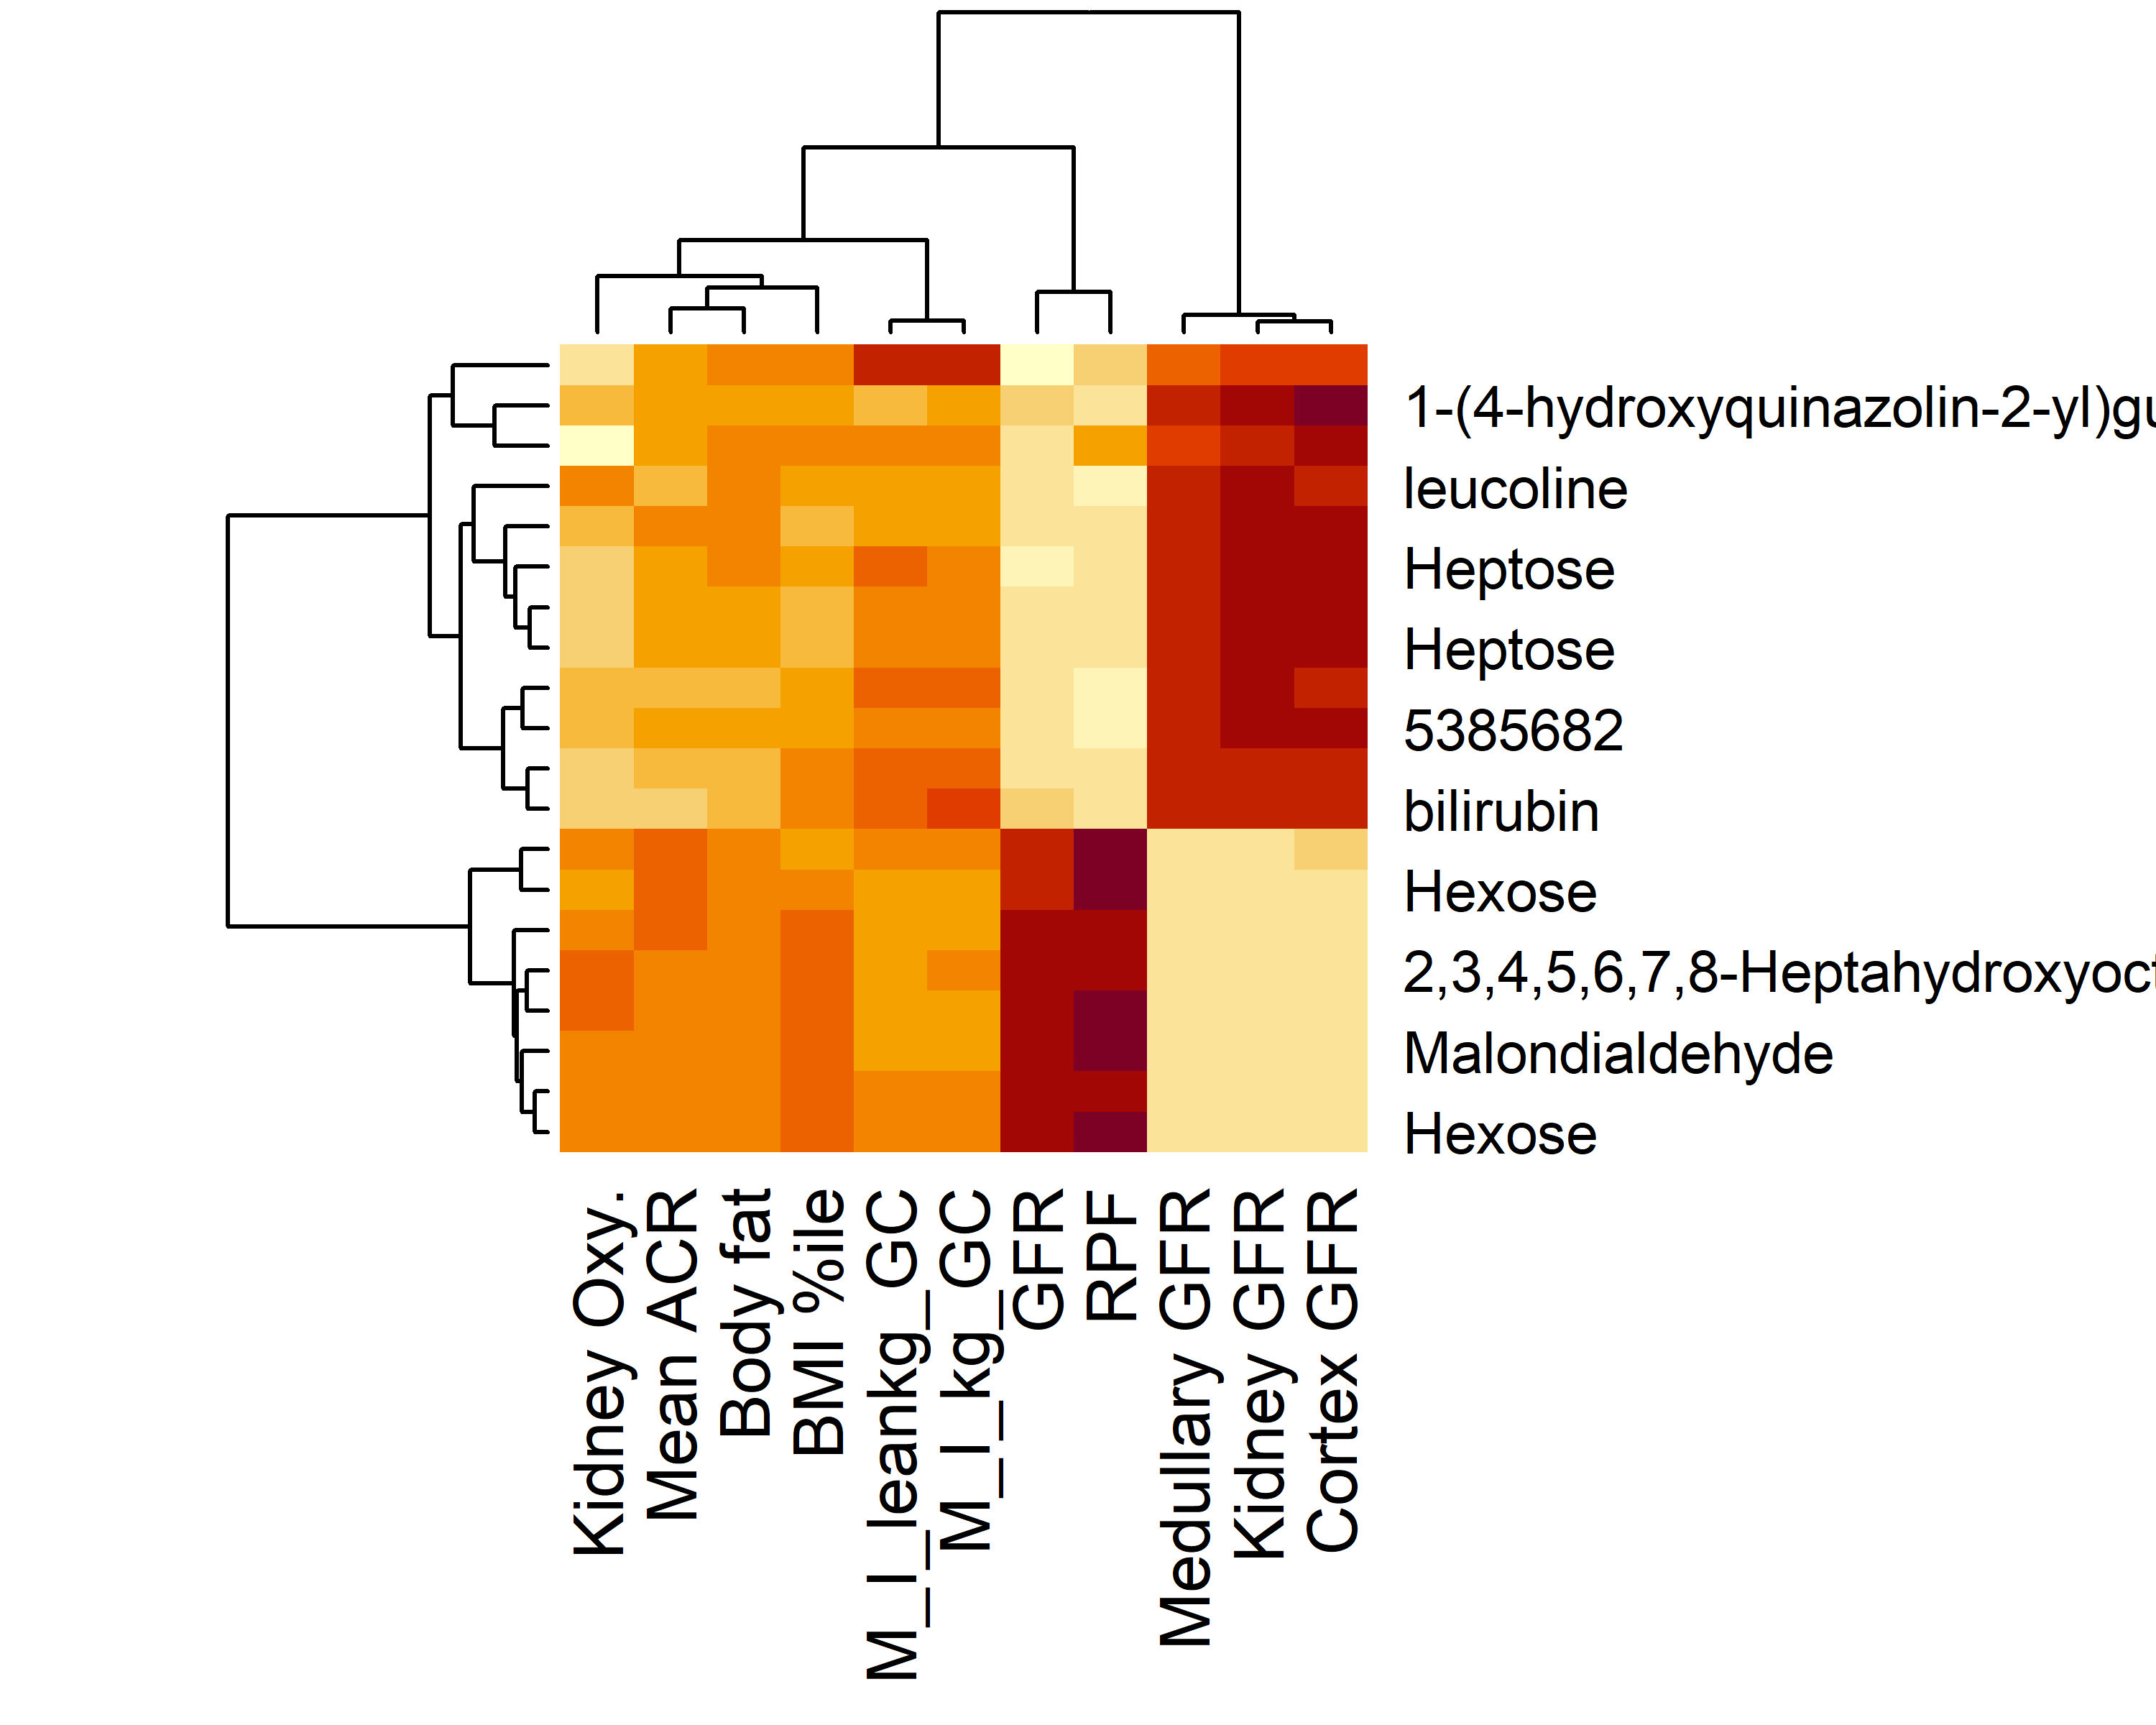
\includegraphics{fat_analysis_pancreatic_fat_files/figure-latex/unnamed-chunk-9-1.pdf}

\begin{longtable}[]{@{}
  >{\raggedright\arraybackslash}p{(\columnwidth - 8\tabcolsep) * \real{0.3247}}
  >{\raggedleft\arraybackslash}p{(\columnwidth - 8\tabcolsep) * \real{0.1429}}
  >{\raggedleft\arraybackslash}p{(\columnwidth - 8\tabcolsep) * \real{0.1429}}
  >{\raggedleft\arraybackslash}p{(\columnwidth - 8\tabcolsep) * \real{0.1429}}
  >{\raggedleft\arraybackslash}p{(\columnwidth - 8\tabcolsep) * \real{0.2468}}@{}}
\caption{T-Table}\tabularnewline
\toprule()
\begin{minipage}[b]{\linewidth}\raggedright
\end{minipage} & \begin{minipage}[b]{\linewidth}\raggedleft
Estimate
\end{minipage} & \begin{minipage}[b]{\linewidth}\raggedleft
Std. Error
\end{minipage} & \begin{minipage}[b]{\linewidth}\raggedleft
t value
\end{minipage} & \begin{minipage}[b]{\linewidth}\raggedleft
Pr(\textgreater\textbar t\textbar)
\end{minipage} \\
\midrule()
\endfirsthead
\toprule()
\begin{minipage}[b]{\linewidth}\raggedright
\end{minipage} & \begin{minipage}[b]{\linewidth}\raggedleft
Estimate
\end{minipage} & \begin{minipage}[b]{\linewidth}\raggedleft
Std. Error
\end{minipage} & \begin{minipage}[b]{\linewidth}\raggedleft
t value
\end{minipage} & \begin{minipage}[b]{\linewidth}\raggedleft
Pr(\textgreater\textbar t\textbar)
\end{minipage} \\
\midrule()
\endhead
study\_phaseNormal Weight & -0.0563636 & 0.4385571 & -0.1285206 &
0.8995650 \\
study\_phaseObese & -0.1960000 & 0.6504853 & -0.3013135 & 0.7676044 \\
\bottomrule()
\end{longtable}

\newpage

\hypertarget{visceral-1}{%
\subsection{visceral}\label{visceral-1}}

\includegraphics{fat_analysis_pancreatic_fat_files/figure-latex/unnamed-chunk-9-2.pdf}

\begin{longtable}[]{@{}
  >{\raggedright\arraybackslash}p{(\columnwidth - 8\tabcolsep) * \real{0.3378}}
  >{\raggedleft\arraybackslash}p{(\columnwidth - 8\tabcolsep) * \real{0.1216}}
  >{\raggedleft\arraybackslash}p{(\columnwidth - 8\tabcolsep) * \real{0.1486}}
  >{\raggedleft\arraybackslash}p{(\columnwidth - 8\tabcolsep) * \real{0.1351}}
  >{\raggedleft\arraybackslash}p{(\columnwidth - 8\tabcolsep) * \real{0.2568}}@{}}
\caption{T-Table}\tabularnewline
\toprule()
\begin{minipage}[b]{\linewidth}\raggedright
\end{minipage} & \begin{minipage}[b]{\linewidth}\raggedleft
Estimate
\end{minipage} & \begin{minipage}[b]{\linewidth}\raggedleft
Std. Error
\end{minipage} & \begin{minipage}[b]{\linewidth}\raggedleft
t value
\end{minipage} & \begin{minipage}[b]{\linewidth}\raggedleft
Pr(\textgreater\textbar t\textbar)
\end{minipage} \\
\midrule()
\endfirsthead
\toprule()
\begin{minipage}[b]{\linewidth}\raggedright
\end{minipage} & \begin{minipage}[b]{\linewidth}\raggedleft
Estimate
\end{minipage} & \begin{minipage}[b]{\linewidth}\raggedleft
Std. Error
\end{minipage} & \begin{minipage}[b]{\linewidth}\raggedleft
t value
\end{minipage} & \begin{minipage}[b]{\linewidth}\raggedleft
Pr(\textgreater\textbar t\textbar)
\end{minipage} \\
\midrule()
\endhead
study\_phaseNormal Weight & 0.385805 & 3.434127 & 0.1123444 &
0.9119477 \\
study\_phaseObese & 8.921998 & 4.856588 & 1.8370917 & 0.0848425 \\
\bottomrule()
\end{longtable}

\newpage

\hypertarget{per_visceral-1}{%
\subsection{per\_visceral}\label{per_visceral-1}}

\includegraphics{fat_analysis_pancreatic_fat_files/figure-latex/unnamed-chunk-9-3.pdf}

\begin{longtable}[]{@{}
  >{\raggedright\arraybackslash}p{(\columnwidth - 8\tabcolsep) * \real{0.3333}}
  >{\raggedleft\arraybackslash}p{(\columnwidth - 8\tabcolsep) * \real{0.1333}}
  >{\raggedleft\arraybackslash}p{(\columnwidth - 8\tabcolsep) * \real{0.1467}}
  >{\raggedleft\arraybackslash}p{(\columnwidth - 8\tabcolsep) * \real{0.1333}}
  >{\raggedleft\arraybackslash}p{(\columnwidth - 8\tabcolsep) * \real{0.2533}}@{}}
\caption{T-Table}\tabularnewline
\toprule()
\begin{minipage}[b]{\linewidth}\raggedright
\end{minipage} & \begin{minipage}[b]{\linewidth}\raggedleft
Estimate
\end{minipage} & \begin{minipage}[b]{\linewidth}\raggedleft
Std. Error
\end{minipage} & \begin{minipage}[b]{\linewidth}\raggedleft
t value
\end{minipage} & \begin{minipage}[b]{\linewidth}\raggedleft
Pr(\textgreater\textbar t\textbar)
\end{minipage} \\
\midrule()
\endfirsthead
\toprule()
\begin{minipage}[b]{\linewidth}\raggedright
\end{minipage} & \begin{minipage}[b]{\linewidth}\raggedleft
Estimate
\end{minipage} & \begin{minipage}[b]{\linewidth}\raggedleft
Std. Error
\end{minipage} & \begin{minipage}[b]{\linewidth}\raggedleft
t value
\end{minipage} & \begin{minipage}[b]{\linewidth}\raggedleft
Pr(\textgreater\textbar t\textbar)
\end{minipage} \\
\midrule()
\endhead
study\_phaseNormal Weight & -1.183830 & 0.4717873 & -2.509244 &
0.0232378 \\
study\_phaseObese & -1.030736 & 0.6672081 & -1.544849 & 0.1419302 \\
\bottomrule()
\end{longtable}

\newpage

\hypertarget{subq_fat-1}{%
\subsection{subq\_fat}\label{subq_fat-1}}

\includegraphics{fat_analysis_pancreatic_fat_files/figure-latex/unnamed-chunk-9-4.pdf}

\begin{longtable}[]{@{}
  >{\raggedright\arraybackslash}p{(\columnwidth - 8\tabcolsep) * \real{0.3425}}
  >{\raggedleft\arraybackslash}p{(\columnwidth - 8\tabcolsep) * \real{0.1233}}
  >{\raggedleft\arraybackslash}p{(\columnwidth - 8\tabcolsep) * \real{0.1507}}
  >{\raggedleft\arraybackslash}p{(\columnwidth - 8\tabcolsep) * \real{0.1233}}
  >{\raggedleft\arraybackslash}p{(\columnwidth - 8\tabcolsep) * \real{0.2603}}@{}}
\caption{T-Table}\tabularnewline
\toprule()
\begin{minipage}[b]{\linewidth}\raggedright
\end{minipage} & \begin{minipage}[b]{\linewidth}\raggedleft
Estimate
\end{minipage} & \begin{minipage}[b]{\linewidth}\raggedleft
Std. Error
\end{minipage} & \begin{minipage}[b]{\linewidth}\raggedleft
t value
\end{minipage} & \begin{minipage}[b]{\linewidth}\raggedleft
Pr(\textgreater\textbar t\textbar)
\end{minipage} \\
\midrule()
\endfirsthead
\toprule()
\begin{minipage}[b]{\linewidth}\raggedright
\end{minipage} & \begin{minipage}[b]{\linewidth}\raggedleft
Estimate
\end{minipage} & \begin{minipage}[b]{\linewidth}\raggedleft
Std. Error
\end{minipage} & \begin{minipage}[b]{\linewidth}\raggedleft
t value
\end{minipage} & \begin{minipage}[b]{\linewidth}\raggedleft
Pr(\textgreater\textbar t\textbar)
\end{minipage} \\
\midrule()
\endhead
study\_phaseNormal Weight & 32.53962 & 11.68917 & 2.783742 &
0.0132791 \\
study\_phaseObese & 80.95554 & 16.53098 & 4.897201 & 0.0001611 \\
\bottomrule()
\end{longtable}

\newpage

\hypertarget{visc_subq_ratio-1}{%
\subsection{visc\_subq\_ratio}\label{visc_subq_ratio-1}}

\includegraphics{fat_analysis_pancreatic_fat_files/figure-latex/unnamed-chunk-9-5.pdf}

\begin{longtable}[]{@{}
  >{\raggedright\arraybackslash}p{(\columnwidth - 8\tabcolsep) * \real{0.3289}}
  >{\raggedleft\arraybackslash}p{(\columnwidth - 8\tabcolsep) * \real{0.1447}}
  >{\raggedleft\arraybackslash}p{(\columnwidth - 8\tabcolsep) * \real{0.1447}}
  >{\raggedleft\arraybackslash}p{(\columnwidth - 8\tabcolsep) * \real{0.1316}}
  >{\raggedleft\arraybackslash}p{(\columnwidth - 8\tabcolsep) * \real{0.2500}}@{}}
\caption{T-Table}\tabularnewline
\toprule()
\begin{minipage}[b]{\linewidth}\raggedright
\end{minipage} & \begin{minipage}[b]{\linewidth}\raggedleft
Estimate
\end{minipage} & \begin{minipage}[b]{\linewidth}\raggedleft
Std. Error
\end{minipage} & \begin{minipage}[b]{\linewidth}\raggedleft
t value
\end{minipage} & \begin{minipage}[b]{\linewidth}\raggedleft
Pr(\textgreater\textbar t\textbar)
\end{minipage} \\
\midrule()
\endfirsthead
\toprule()
\begin{minipage}[b]{\linewidth}\raggedright
\end{minipage} & \begin{minipage}[b]{\linewidth}\raggedleft
Estimate
\end{minipage} & \begin{minipage}[b]{\linewidth}\raggedleft
Std. Error
\end{minipage} & \begin{minipage}[b]{\linewidth}\raggedleft
t value
\end{minipage} & \begin{minipage}[b]{\linewidth}\raggedleft
Pr(\textgreater\textbar t\textbar)
\end{minipage} \\
\midrule()
\endhead
study\_phaseNormal Weight & -0.0895298 & 0.0143717 & -6.229601 &
0.0000120 \\
study\_phaseObese & -0.0297938 & 0.0203246 & -1.465896 & 0.1620532 \\
\bottomrule()
\end{longtable}

\newpage

\hypertarget{fat_percentage_dexa-1}{%
\subsection{fat\_percentage\_dexa}\label{fat_percentage_dexa-1}}

\includegraphics{fat_analysis_pancreatic_fat_files/figure-latex/unnamed-chunk-9-6.pdf}

\begin{longtable}[]{@{}
  >{\raggedright\arraybackslash}p{(\columnwidth - 8\tabcolsep) * \real{0.3247}}
  >{\raggedleft\arraybackslash}p{(\columnwidth - 8\tabcolsep) * \real{0.1429}}
  >{\raggedleft\arraybackslash}p{(\columnwidth - 8\tabcolsep) * \real{0.1429}}
  >{\raggedleft\arraybackslash}p{(\columnwidth - 8\tabcolsep) * \real{0.1429}}
  >{\raggedleft\arraybackslash}p{(\columnwidth - 8\tabcolsep) * \real{0.2468}}@{}}
\caption{T-Table}\tabularnewline
\toprule()
\begin{minipage}[b]{\linewidth}\raggedright
\end{minipage} & \begin{minipage}[b]{\linewidth}\raggedleft
Estimate
\end{minipage} & \begin{minipage}[b]{\linewidth}\raggedleft
Std. Error
\end{minipage} & \begin{minipage}[b]{\linewidth}\raggedleft
t value
\end{minipage} & \begin{minipage}[b]{\linewidth}\raggedleft
Pr(\textgreater\textbar t\textbar)
\end{minipage} \\
\midrule()
\endfirsthead
\toprule()
\begin{minipage}[b]{\linewidth}\raggedright
\end{minipage} & \begin{minipage}[b]{\linewidth}\raggedleft
Estimate
\end{minipage} & \begin{minipage}[b]{\linewidth}\raggedleft
Std. Error
\end{minipage} & \begin{minipage}[b]{\linewidth}\raggedleft
t value
\end{minipage} & \begin{minipage}[b]{\linewidth}\raggedleft
Pr(\textgreater\textbar t\textbar)
\end{minipage} \\
\midrule()
\endhead
study\_phaseNormal Weight & -0.6083333 & 1.123658 & -0.5413867 &
0.5961911 \\
study\_phaseObese & -0.8000000 & 1.740763 & -0.4595686 & 0.6524161 \\
\bottomrule()
\end{longtable}

\newpage

\hypertarget{lept-1}{%
\subsection{lept}\label{lept-1}}

\includegraphics{fat_analysis_pancreatic_fat_files/figure-latex/unnamed-chunk-9-7.pdf}

\begin{longtable}[]{@{}
  >{\raggedright\arraybackslash}p{(\columnwidth - 8\tabcolsep) * \real{0.3378}}
  >{\raggedleft\arraybackslash}p{(\columnwidth - 8\tabcolsep) * \real{0.1351}}
  >{\raggedleft\arraybackslash}p{(\columnwidth - 8\tabcolsep) * \real{0.1486}}
  >{\raggedleft\arraybackslash}p{(\columnwidth - 8\tabcolsep) * \real{0.1216}}
  >{\raggedleft\arraybackslash}p{(\columnwidth - 8\tabcolsep) * \real{0.2568}}@{}}
\caption{T-Table}\tabularnewline
\toprule()
\begin{minipage}[b]{\linewidth}\raggedright
\end{minipage} & \begin{minipage}[b]{\linewidth}\raggedleft
Estimate
\end{minipage} & \begin{minipage}[b]{\linewidth}\raggedleft
Std. Error
\end{minipage} & \begin{minipage}[b]{\linewidth}\raggedleft
t value
\end{minipage} & \begin{minipage}[b]{\linewidth}\raggedleft
Pr(\textgreater\textbar t\textbar)
\end{minipage} \\
\midrule()
\endfirsthead
\toprule()
\begin{minipage}[b]{\linewidth}\raggedright
\end{minipage} & \begin{minipage}[b]{\linewidth}\raggedleft
Estimate
\end{minipage} & \begin{minipage}[b]{\linewidth}\raggedleft
Std. Error
\end{minipage} & \begin{minipage}[b]{\linewidth}\raggedleft
t value
\end{minipage} & \begin{minipage}[b]{\linewidth}\raggedleft
Pr(\textgreater\textbar t\textbar)
\end{minipage} \\
\midrule()
\endhead
study\_phaseNormal Weight & 2.858333 & 3.083713 & 0.926913 &
0.3677434 \\
study\_phaseObese & 21.266667 & 4.361028 & 4.876526 & 0.0001680 \\
\bottomrule()
\end{longtable}

\newpage

\hypertarget{ast-1}{%
\subsection{ast}\label{ast-1}}

\includegraphics{fat_analysis_pancreatic_fat_files/figure-latex/unnamed-chunk-9-8.pdf}

\begin{longtable}[]{@{}
  >{\raggedright\arraybackslash}p{(\columnwidth - 8\tabcolsep) * \real{0.3333}}
  >{\raggedleft\arraybackslash}p{(\columnwidth - 8\tabcolsep) * \real{0.1333}}
  >{\raggedleft\arraybackslash}p{(\columnwidth - 8\tabcolsep) * \real{0.1467}}
  >{\raggedleft\arraybackslash}p{(\columnwidth - 8\tabcolsep) * \real{0.1333}}
  >{\raggedleft\arraybackslash}p{(\columnwidth - 8\tabcolsep) * \real{0.2533}}@{}}
\caption{T-Table}\tabularnewline
\toprule()
\begin{minipage}[b]{\linewidth}\raggedright
\end{minipage} & \begin{minipage}[b]{\linewidth}\raggedleft
Estimate
\end{minipage} & \begin{minipage}[b]{\linewidth}\raggedleft
Std. Error
\end{minipage} & \begin{minipage}[b]{\linewidth}\raggedleft
t value
\end{minipage} & \begin{minipage}[b]{\linewidth}\raggedleft
Pr(\textgreater\textbar t\textbar)
\end{minipage} \\
\midrule()
\endfirsthead
\toprule()
\begin{minipage}[b]{\linewidth}\raggedright
\end{minipage} & \begin{minipage}[b]{\linewidth}\raggedleft
Estimate
\end{minipage} & \begin{minipage}[b]{\linewidth}\raggedleft
Std. Error
\end{minipage} & \begin{minipage}[b]{\linewidth}\raggedleft
t value
\end{minipage} & \begin{minipage}[b]{\linewidth}\raggedleft
Pr(\textgreater\textbar t\textbar)
\end{minipage} \\
\midrule()
\endhead
study\_phaseNormal Weight & -12.66667 & 5.43746 & -2.329519 &
0.0332546 \\
study\_phaseObese & -11.00000 & 7.68973 & -1.430479 & 0.1718189 \\
\bottomrule()
\end{longtable}

\newpage

\hypertarget{alt-1}{%
\subsection{alt}\label{alt-1}}

\includegraphics{fat_analysis_pancreatic_fat_files/figure-latex/unnamed-chunk-9-9.pdf}

\begin{longtable}[]{@{}
  >{\raggedright\arraybackslash}p{(\columnwidth - 8\tabcolsep) * \real{0.3289}}
  >{\raggedleft\arraybackslash}p{(\columnwidth - 8\tabcolsep) * \real{0.1447}}
  >{\raggedleft\arraybackslash}p{(\columnwidth - 8\tabcolsep) * \real{0.1447}}
  >{\raggedleft\arraybackslash}p{(\columnwidth - 8\tabcolsep) * \real{0.1316}}
  >{\raggedleft\arraybackslash}p{(\columnwidth - 8\tabcolsep) * \real{0.2500}}@{}}
\caption{T-Table}\tabularnewline
\toprule()
\begin{minipage}[b]{\linewidth}\raggedright
\end{minipage} & \begin{minipage}[b]{\linewidth}\raggedleft
Estimate
\end{minipage} & \begin{minipage}[b]{\linewidth}\raggedleft
Std. Error
\end{minipage} & \begin{minipage}[b]{\linewidth}\raggedleft
t value
\end{minipage} & \begin{minipage}[b]{\linewidth}\raggedleft
Pr(\textgreater\textbar t\textbar)
\end{minipage} \\
\midrule()
\endfirsthead
\toprule()
\begin{minipage}[b]{\linewidth}\raggedright
\end{minipage} & \begin{minipage}[b]{\linewidth}\raggedleft
Estimate
\end{minipage} & \begin{minipage}[b]{\linewidth}\raggedleft
Std. Error
\end{minipage} & \begin{minipage}[b]{\linewidth}\raggedleft
t value
\end{minipage} & \begin{minipage}[b]{\linewidth}\raggedleft
Pr(\textgreater\textbar t\textbar)
\end{minipage} \\
\midrule()
\endhead
study\_phaseNormal Weight & -8.9166667 & 2.249711 & -3.963473 &
0.0011144 \\
study\_phaseObese & 0.1666667 & 3.181571 & 0.052385 & 0.9588704 \\
\bottomrule()
\end{longtable}

\hypertarget{delta-models---t-tests}{%
\section{Delta Models - T-tests}\label{delta-models---t-tests}}

T-tests stratified by group.

\hypertarget{pancreatic_fat_avg-2}{%
\subsection{pancreatic\_fat\_AVG}\label{pancreatic_fat_avg-2}}

\begin{longtable}[]{@{}lrr@{}}
\caption{T-test Results}\tabularnewline
\toprule()
group & estimate & p \\
\midrule()
\endfirsthead
\toprule()
group & estimate & p \\
\midrule()
\endhead
Normal Weight & -0.0563636 & 0.9011266 \\
Obese & -0.1960000 & 0.7734484 \\
\bottomrule()
\end{longtable}

\hypertarget{visceral-2}{%
\subsection{visceral}\label{visceral-2}}

\begin{longtable}[]{@{}lrr@{}}
\caption{T-test Results}\tabularnewline
\toprule()
group & estimate & p \\
\midrule()
\endfirsthead
\toprule()
group & estimate & p \\
\midrule()
\endhead
Normal Weight & 0.385805 & 0.8373515 \\
Obese & 8.921998 & 0.3038178 \\
\bottomrule()
\end{longtable}

\hypertarget{per_visceral-2}{%
\subsection{per\_visceral}\label{per_visceral-2}}

\begin{longtable}[]{@{}lrr@{}}
\caption{T-test Results}\tabularnewline
\toprule()
group & estimate & p \\
\midrule()
\endfirsthead
\toprule()
group & estimate & p \\
\midrule()
\endhead
Normal Weight & -1.183830 & 0.0188941 \\
Obese & -1.030736 & 0.2438133 \\
\bottomrule()
\end{longtable}

\hypertarget{subq_fat-2}{%
\subsection{subq\_fat}\label{subq_fat-2}}

\begin{longtable}[]{@{}lrr@{}}
\caption{T-test Results}\tabularnewline
\toprule()
group & estimate & p \\
\midrule()
\endfirsthead
\toprule()
group & estimate & p \\
\midrule()
\endhead
Normal Weight & 32.53962 & 0.0219858 \\
Obese & 80.95554 & 0.0027675 \\
\bottomrule()
\end{longtable}

\hypertarget{visc_subq_ratio-2}{%
\subsection{visc\_subq\_ratio}\label{visc_subq_ratio-2}}

\begin{longtable}[]{@{}lrr@{}}
\caption{T-test Results}\tabularnewline
\toprule()
group & estimate & p \\
\midrule()
\endfirsthead
\toprule()
group & estimate & p \\
\midrule()
\endhead
Normal Weight & -0.0895298 & 0.0001294 \\
Obese & -0.0297938 & 0.1199828 \\
\bottomrule()
\end{longtable}

\hypertarget{fat_percentage_dexa-2}{%
\subsection{fat\_percentage\_dexa}\label{fat_percentage_dexa-2}}

\begin{longtable}[]{@{}lrr@{}}
\caption{T-test Results}\tabularnewline
\toprule()
group & estimate & p \\
\midrule()
\endfirsthead
\toprule()
group & estimate & p \\
\midrule()
\endhead
Normal Weight & -0.6083333 & 0.5772197 \\
Obese & -0.8000000 & 0.7082967 \\
\bottomrule()
\end{longtable}

\hypertarget{lept-2}{%
\subsection{lept}\label{lept-2}}

\begin{longtable}[]{@{}lrr@{}}
\caption{T-test Results}\tabularnewline
\toprule()
group & estimate & p \\
\midrule()
\endfirsthead
\toprule()
group & estimate & p \\
\midrule()
\endhead
Normal Weight & 2.858333 & 0.0837741 \\
Obese & 21.266667 & 0.0307847 \\
\bottomrule()
\end{longtable}

\hypertarget{ast-2}{%
\subsection{ast}\label{ast-2}}

\begin{longtable}[]{@{}lrr@{}}
\caption{T-test Results}\tabularnewline
\toprule()
group & estimate & p \\
\midrule()
\endfirsthead
\toprule()
group & estimate & p \\
\midrule()
\endhead
Normal Weight & -12.66667 & 0.0599219 \\
Obese & -11.00000 & 0.0950977 \\
\bottomrule()
\end{longtable}

\hypertarget{alt-2}{%
\subsection{alt}\label{alt-2}}

\begin{longtable}[]{@{}lrr@{}}
\caption{T-test Results}\tabularnewline
\toprule()
group & estimate & p \\
\midrule()
\endfirsthead
\toprule()
group & estimate & p \\
\midrule()
\endhead
Normal Weight & -8.9166667 & 0.0000532 \\
Obese & 0.1666667 & 0.9740476 \\
\bottomrule()
\end{longtable}

\hypertarget{multivariable-models}{%
\section{Multivariable Models}\label{multivariable-models}}

Models are fitted using important variables selected by Elastic Net
models.

\hypertarget{predict-tanner-5-pancreatic-fat-with-tanner-5-covariates}{%
\subsection{Predict Tanner 5 Pancreatic Fat with Tanner 5
Covariates}\label{predict-tanner-5-pancreatic-fat-with-tanner-5-covariates}}

Variables Considered:

\begin{verbatim}
##  [1] "insulin_secretion_mm" "insulin_sensitivity"  "tg_lv"               
##  [4] "crp_lv"               "hba"                  "igf_lv"              
##  [7] "sex_exam"             "race_eth"             "pancreatic_fat_AVG"  
## [10] "visceral"             "per_visceral"         "subq_fat"            
## [13] "visc_subq_ratio"      "fat_percentage_dexa"  "lept"                
## [16] "lept_adipo_ratio"     "estradiol"            "total_testosterone"  
## [19] "shbg"                 "fasting_glucose"      "fasting_insulin"
\end{verbatim}

\hypertarget{with-obesity}{%
\subsubsection{With obesity}\label{with-obesity}}

\begin{verbatim}
## Anova Table (Type III tests)
## 
## Response: pancreatic_fat_AVG
##                      Sum Sq Df F value Pr(>F)
## (Intercept)          2.2042  1  2.8812 0.1882
## study_phase          0.2018  1  0.2637 0.6430
## lept                 0.1051  1  0.1374 0.7355
## lept_adipo_ratio     0.2027  1  0.2650 0.6422
## hba                  2.2372  1  2.9242 0.1858
## crp_lv               0.0531  1  0.0694 0.8092
## insulin_secretion_mm 0.0039  1  0.0051 0.9475
## fasting_glucose      0.6237  1  0.8153 0.4331
## race_eth             3.2711  4  1.0689 0.4982
## shbg                 0.1401  1  0.1831 0.6976
## per_visceral         0.0191  1  0.0250 0.8845
## visc_subq_ratio      0.0002  1  0.0003 0.9875
## Residuals            2.2951  3
\end{verbatim}

\begin{verbatim}
## 
## Call:
## lm(formula = pancreatic_fat_AVG ~ study_phase + lept + lept_adipo_ratio + 
##     hba + crp_lv + insulin_secretion_mm + fasting_glucose + race_eth + 
##     shbg + per_visceral + visc_subq_ratio, data = dat_t5, na.action = na.omit)
## 
## Residuals:
##          3          4          5          6          7          8          9 
## -4.788e-02  2.651e-01 -2.651e-01  2.651e-01  8.674e-18 -2.766e-02 -6.912e-01 
##         10         11         12         13         14         15         16 
##  6.147e-01  1.998e-01 -5.871e-01 -8.089e-02  1.701e-01  7.537e-01 -3.515e-01 
##         17         19         20         22 
## -2.601e-01 -1.593e-01  8.966e-02  1.125e-01 
## 
## Coefficients:
##                        Estimate Std. Error t value Pr(>|t|)
## (Intercept)          -1.381e+01  8.134e+00  -1.697    0.188
## study_phaseObese     -9.346e-01  1.820e+00  -0.514    0.643
## lept                 -4.632e-02  1.250e-01  -0.371    0.736
## lept_adipo_ratio      4.073e-01  7.912e-01   0.515    0.642
## hba                   1.679e+00  9.816e-01   1.710    0.186
## crp_lv                4.249e-02  1.613e-01   0.263    0.809
## insulin_secretion_mm  2.705e-05  3.782e-04   0.072    0.947
## fasting_glucose       7.094e-02  7.856e-02   0.903    0.433
## race_ethNHW          -7.507e-02  1.450e+00  -0.052    0.962
## race_ethBlack         1.136e+00  3.099e+00   0.367    0.738
## race_ethAsian        -5.542e-01  1.558e+00  -0.356    0.746
## race_ethOther         1.591e+00  1.548e+00   1.028    0.380
## shbg                  9.298e-03  2.173e-02   0.428    0.698
## per_visceral         -1.985e-02  1.256e-01  -0.158    0.884
## visc_subq_ratio      -5.368e-02  3.158e+00  -0.017    0.988
## 
## Residual standard error: 0.8747 on 3 degrees of freedom
##   (5 observations deleted due to missingness)
## Multiple R-squared:  0.9202, Adjusted R-squared:  0.548 
## F-statistic: 2.472 on 14 and 3 DF,  p-value: 0.2479
\end{verbatim}

\hypertarget{without-obesity}{%
\subsubsection{Without obesity}\label{without-obesity}}

\begin{verbatim}
## Anova Table (Type III tests)
## 
## Response: pancreatic_fat_AVG
##                      Sum Sq Df F value  Pr(>F)  
## (Intercept)          2.3664  1  3.7910 0.12338  
## lept                 0.0556  1  0.0890 0.78027  
## lept_adipo_ratio     0.1139  1  0.1824 0.69131  
## hba                  3.2840  1  5.2610 0.08352 .
## crp_lv               0.0486  1  0.0778 0.79415  
## insulin_secretion_mm 0.0000  1  0.0000 0.99677  
## fasting_glucose      0.4720  1  0.7561 0.43363  
## race_eth             3.0830  4  1.2347 0.42151  
## shbg                 0.5071  1  0.8123 0.41839  
## per_visceral         0.1238  1  0.1984 0.67909  
## visc_subq_ratio      0.0018  1  0.0029 0.95959  
## Residuals            2.4969  4                  
## ---
## Signif. codes:  0 '***' 0.001 '**' 0.01 '*' 0.05 '.' 0.1 ' ' 1
\end{verbatim}

\begin{verbatim}
## 
## Call:
## lm(formula = pancreatic_fat_AVG ~ lept + lept_adipo_ratio + hba + 
##     crp_lv + insulin_secretion_mm + fasting_glucose + race_eth + 
##     shbg + per_visceral + visc_subq_ratio, data = dat_t5, na.action = na.omit)
## 
## Residuals:
##          3          4          5          6          7          8          9 
## -3.085e-01  4.113e-01 -1.954e-01  1.954e-01  1.388e-17 -1.353e-01 -6.003e-01 
##         10         11         12         13         14         15         16 
##  6.785e-01  2.629e-01 -5.432e-01 -6.395e-02  2.591e-01  7.041e-01 -5.618e-01 
##         17         19         20         22 
## -1.526e-01 -1.514e-01  1.457e-01  5.547e-02 
## 
## Coefficients:
##                        Estimate Std. Error t value Pr(>|t|)  
## (Intercept)          -1.423e+01  7.309e+00  -1.947   0.1234  
## lept                 -3.294e-02  1.104e-01  -0.298   0.7803  
## lept_adipo_ratio      2.928e-01  6.857e-01   0.427   0.6913  
## hba                   1.874e+00  8.171e-01   2.294   0.0835 .
## crp_lv                4.062e-02  1.456e-01   0.279   0.7941  
## insulin_secretion_mm -1.457e-06  3.379e-04  -0.004   0.9968  
## fasting_glucose       5.889e-02  6.773e-02   0.870   0.4336  
## race_ethNHW           3.006e-01  1.131e+00   0.266   0.8035  
## race_ethBlack         1.000e+00  2.789e+00   0.359   0.7380  
## race_ethAsian        -3.783e-02  1.075e+00  -0.035   0.9736  
## race_ethOther         1.847e+00  1.323e+00   1.396   0.2353  
## shbg                  1.511e-02  1.676e-02   0.901   0.4184  
## per_visceral         -4.613e-02  1.036e-01  -0.445   0.6791  
## visc_subq_ratio      -1.535e-01  2.847e+00  -0.054   0.9596  
## ---
## Signif. codes:  0 '***' 0.001 '**' 0.01 '*' 0.05 '.' 0.1 ' ' 1
## 
## Residual standard error: 0.7901 on 4 degrees of freedom
##   (5 observations deleted due to missingness)
## Multiple R-squared:  0.9132, Adjusted R-squared:  0.6312 
## F-statistic: 3.238 on 13 and 4 DF,  p-value: 0.133
\end{verbatim}

\hypertarget{predict-tanner-23-pancreatic-fat-with-tanner-23-covariates}{%
\subsection{Predict Tanner 2/3 Pancreatic Fat with Tanner 2/3
Covariates}\label{predict-tanner-23-pancreatic-fat-with-tanner-23-covariates}}

Variables Considered:

\begin{verbatim}
##  [1] "insulin_secretion_mm" "insulin_sensitivity"  "tg_lv"               
##  [4] "crp_lv"               "hba"                  "igf_lv"              
##  [7] "sex_exam"             "race_eth"             "pancreatic_fat_AVG"  
## [10] "visceral"             "per_visceral"         "subq_fat"            
## [13] "visc_subq_ratio"      "fat_percentage_dexa"  "lept"                
## [16] "lept_adipo_ratio"     "estradiol"            "total_testosterone"  
## [19] "shbg"                 "fasting_glucose"      "fasting_insulin"     
## [22] "study_phase"
\end{verbatim}

\hypertarget{with-obesity-1}{%
\subsubsection{with obesity}\label{with-obesity-1}}

\begin{verbatim}
## Anova Table (Type III tests)
## 
## Response: pancreatic_fat_AVG
##                      Sum Sq Df F value Pr(>F)
## (Intercept)          0.0117  1  0.0059 0.9423
## study_phase          0.7984  1  0.4054 0.5589
## lept                 0.2185  1  0.1110 0.7558
## race_eth             5.3041  4  0.6734 0.6445
## hba                  0.1950  1  0.0990 0.7687
## insulin_secretion_mm 1.1543  1  0.5862 0.4866
## visceral             0.3136  1  0.1592 0.7103
## lept_adipo_ratio     0.0231  1  0.0117 0.9189
## tg_lv                0.3393  1  0.1723 0.6994
## estradiol            0.1378  1  0.0700 0.8044
## Residuals            7.8767  4
\end{verbatim}

\begin{verbatim}
## 
## Call:
## lm(formula = pancreatic_fat_AVG ~ study_phase + lept + race_eth + 
##     hba + insulin_secretion_mm + visceral + lept_adipo_ratio + 
##     tg_lv + estradiol, data = fat_measures_baseline, na.action = na.omit)
## 
## Residuals:
##        1        3        4        5        6        7        8        9 
## -0.32516 -0.32516  0.32516  0.32516  0.86762 -0.85879 -0.03926  0.74954 
##       10       11       13       14       15       18       19       20 
## -0.82836  1.10247 -1.30933  1.03441 -0.71830  0.24451 -0.34909  0.12690 
##       23 
## -0.02232 
## 
## Coefficients:
##                       Estimate Std. Error t value Pr(>|t|)
## (Intercept)          -1.035346  13.434697  -0.077    0.942
## study_phaseObese      2.560401   4.021174   0.637    0.559
## lept                  0.071295   0.214010   0.333    0.756
## race_ethNHW          -0.705479   4.342623  -0.162    0.879
## race_ethBlack         2.553034   2.661157   0.959    0.392
## race_ethAsian         0.240405   3.524254   0.068    0.949
## race_ethOther         0.215417   2.193475   0.098    0.926
## hba                   0.580664   1.845183   0.315    0.769
## insulin_secretion_mm -0.001902   0.002484  -0.766    0.487
## visceral              0.013782   0.034539   0.399    0.710
## lept_adipo_ratio      0.051286   0.473380   0.108    0.919
## tg_lv                -0.005369   0.012934  -0.415    0.699
## estradiol             0.032026   0.121053   0.265    0.804
## 
## Residual standard error: 1.403 on 4 degrees of freedom
##   (7 observations deleted due to missingness)
## Multiple R-squared:  0.7864, Adjusted R-squared:  0.1454 
## F-statistic: 1.227 on 12 and 4 DF,  p-value: 0.4605
\end{verbatim}

\hypertarget{without-obesity-1}{%
\subsubsection{without obesity}\label{without-obesity-1}}

\begin{verbatim}
## Anova Table (Type III tests)
## 
## Response: pancreatic_fat_AVG
##                      Sum Sq Df F value Pr(>F)
## (Intercept)          0.5007  1  0.2886 0.6142
## lept                 1.4740  1  0.8496 0.3990
## race_eth             9.8036  4  1.4126 0.3513
## hba                  0.0109  1  0.0063 0.9398
## insulin_secretion_mm 4.3979  1  2.5348 0.1722
## visceral             0.7599  1  0.4380 0.5374
## lept_adipo_ratio     1.3119  1  0.7561 0.4243
## tg_lv                1.2582  1  0.7252 0.4333
## estradiol            0.1430  1  0.0824 0.7856
## Residuals            8.6751  5
\end{verbatim}

\begin{verbatim}
## 
## Call:
## lm(formula = pancreatic_fat_AVG ~ lept + race_eth + hba + insulin_secretion_mm + 
##     visceral + lept_adipo_ratio + tg_lv + estradiol, data = fat_measures_baseline, 
##     na.action = na.omit)
## 
## Residuals:
##       1       3       4       5       6       7       8       9      10      11 
## -0.2439 -0.5557  0.5557  0.2439  0.6966 -0.7577  0.1941  0.2632 -0.8907  1.3665 
##      13      14      15      18      19      20      23 
## -1.5617  1.0856 -0.3959  0.3759 -0.4038 -0.1132  0.1411 
## 
## Coefficients:
##                       Estimate Std. Error t value Pr(>|t|)
## (Intercept)           4.887633   9.098743   0.537    0.614
## lept                  0.150586   0.163374   0.922    0.399
## race_ethNHW          -2.948664   2.383349  -1.237    0.271
## race_ethBlack         1.725020   2.179367   0.792    0.465
## race_ethAsian        -1.693343   1.678341  -1.009    0.359
## race_ethOther        -0.492971   1.774439  -0.278    0.792
## hba                  -0.111069   1.399982  -0.079    0.940
## insulin_secretion_mm -0.002893   0.001817  -1.592    0.172
## visceral              0.020446   0.030896   0.662    0.537
## lept_adipo_ratio      0.268233   0.308473   0.870    0.424
## tg_lv                -0.009171   0.010769  -0.852    0.433
## estradiol             0.032617   0.113624   0.287    0.786
## 
## Residual standard error: 1.317 on 5 degrees of freedom
##   (7 observations deleted due to missingness)
## Multiple R-squared:  0.7647, Adjusted R-squared:  0.2471 
## F-statistic: 1.477 on 11 and 5 DF,  p-value: 0.3501
\end{verbatim}

\hypertarget{predict-tanner-5-pancreatic-fat-with-tanner-23-covariates}{%
\subsection{Predict Tanner 5 Pancreatic Fat with Tanner 2/3
Covariates}\label{predict-tanner-5-pancreatic-fat-with-tanner-23-covariates}}

Variables Considered:

\begin{verbatim}
##  [1] "sex_exam"                      "race_eth"                     
##  [3] "baseline_insulin_secretion_mm" "baseline_insulin_sensitivity" 
##  [5] "baseline_tg_lv"                "baseline_crp_lv"              
##  [7] "baseline_hba"                  "baseline_igf_lv"              
##  [9] "baseline_lept_adipo_ratio"     "baseline_pancreatic_fat_AVG"  
## [11] "baseline_visceral"             "baseline_per_visceral"        
## [13] "baseline_subq_fat"             "baseline_visc_subq_ratio"     
## [15] "baseline_fat_percentage_dexa"  "baseline_lept"                
## [17] "baseline_estradiol"            "baseline_total_testosterone"  
## [19] "baseline_shbg"                 "baseline_fasting_glucose"     
## [21] "baseline_fasting_insulin"
\end{verbatim}

\hypertarget{with-obesity-2}{%
\subsubsection{with obesity}\label{with-obesity-2}}

\begin{verbatim}
## Anova Table (Type III tests)
## 
## Response: pancreatic_fat_AVG
##                             Sum Sq Df F value  Pr(>F)  
## (Intercept)                 0.4078  1  6.1715 0.13095  
## study_phase                 0.6172  1  9.3402 0.09246 .
## baseline_pancreatic_fat_AVG 0.8638  1 13.0731 0.06870 .
## baseline_fasting_insulin    1.3351  1 20.2059 0.04610 *
## race_eth                    8.1640  4 30.8892 0.03160 *
## baseline_shbg               2.2475  1 34.0142 0.02816 *
## baseline_lept_adipo_ratio   0.2897  1  4.3844 0.17130  
## baseline_visc_subq_ratio    0.3583  1  5.4222 0.14529  
## baseline_crp_lv             0.3170  1  4.7983 0.15988  
## baseline_visceral           0.8322  1 12.5950 0.07104 .
## sex_exam                    1.0400  1 15.7403 0.05805 .
## Residuals                   0.1322  2                  
## ---
## Signif. codes:  0 '***' 0.001 '**' 0.01 '*' 0.05 '.' 0.1 ' ' 1
\end{verbatim}

\begin{verbatim}
## 
## Call:
## lm(formula = pancreatic_fat_AVG ~ study_phase + baseline_pancreatic_fat_AVG + 
##     baseline_fasting_insulin + race_eth + baseline_shbg + baseline_lept_adipo_ratio + 
##     baseline_visc_subq_ratio + baseline_crp_lv + baseline_visceral + 
##     sex_exam, data = dat_t5, na.action = na.omit)
## 
## Residuals:
##          5          6          7          8          9         10         11 
## -2.082e-17 -7.633e-18  6.578e-18  1.537e-01  3.762e-02 -3.750e-02 -1.657e-02 
##         12         13         14         15         16         17         19 
## -1.162e-01 -1.844e-01 -1.038e-01  1.243e-01  1.428e-01  1.348e-02  7.810e-02 
##         20         22 
## -2.533e-02 -6.626e-02 
## 
## Coefficients:
##                              Estimate Std. Error t value Pr(>|t|)  
## (Intercept)                   6.17097    2.48404   2.484   0.1310  
## study_phaseObese             -7.06438    2.31151  -3.056   0.0925 .
## baseline_pancreatic_fat_AVG   0.51392    0.14214   3.616   0.0687 .
## baseline_fasting_insulin     -0.06198    0.01379  -4.495   0.0461 *
## race_ethNHW                 -10.84750    2.77839  -3.904   0.0598 .
## race_ethBlack               -10.59013    2.88242  -3.674   0.0667 .
## race_ethAsian                -7.90616    2.38811  -3.311   0.0804 .
## race_ethOther                -4.45273    2.23637  -1.991   0.1847  
## baseline_shbg                 0.07752    0.01329   5.832   0.0282 *
## baseline_lept_adipo_ratio    -0.42781    0.20431  -2.094   0.1713  
## baseline_visc_subq_ratio     -5.47215    2.35002  -2.329   0.1453  
## baseline_crp_lv               1.40538    0.64158   2.190   0.1599  
## baseline_visceral             0.04117    0.01160   3.549   0.0710 .
## sex_examMale                  1.32876    0.33492   3.967   0.0581 .
## ---
## Signif. codes:  0 '***' 0.001 '**' 0.01 '*' 0.05 '.' 0.1 ' ' 1
## 
## Residual standard error: 0.2571 on 2 degrees of freedom
##   (7 observations deleted due to missingness)
## Multiple R-squared:  0.995,  Adjusted R-squared:  0.9622 
## F-statistic: 30.41 on 13 and 2 DF,  p-value: 0.03227
\end{verbatim}

\hypertarget{without-obesity-2}{%
\subsubsection{without obesity}\label{without-obesity-2}}

\begin{verbatim}
## Anova Table (Type III tests)
## 
## Response: pancreatic_fat_AVG
##                             Sum Sq Df F value  Pr(>F)  
## (Intercept)                 0.1025  1  0.4103 0.56738  
## baseline_pancreatic_fat_AVG 0.2631  1  1.0533 0.38028  
## baseline_fasting_insulin    1.1134  1  4.4577 0.12521  
## race_eth                    8.3645  4  8.3722 0.05603 .
## baseline_shbg               2.2626  1  9.0587 0.05722 .
## baseline_lept_adipo_ratio   0.1593  1  0.6379 0.48285  
## baseline_visc_subq_ratio    0.0455  1  0.1821 0.69834  
## baseline_crp_lv             0.0888  1  0.3557 0.59291  
## baseline_visceral           0.8020  1  3.2111 0.17105  
## sex_exam                    0.4231  1  1.6941 0.28399  
## Residuals                   0.7493  3                  
## ---
## Signif. codes:  0 '***' 0.001 '**' 0.01 '*' 0.05 '.' 0.1 ' ' 1
\end{verbatim}

\begin{verbatim}
## 
## Call:
## lm(formula = pancreatic_fat_AVG ~ baseline_pancreatic_fat_AVG + 
##     baseline_fasting_insulin + race_eth + baseline_shbg + baseline_lept_adipo_ratio + 
##     baseline_visc_subq_ratio + baseline_crp_lv + baseline_visceral + 
##     sex_exam, data = fat_measures_tanner5_w_baseline, na.action = na.omit)
## 
## Residuals:
##          5          6          7          8          9         10         11 
##  8.736e-02 -8.736e-02  4.857e-17  1.293e-01  1.205e-01 -6.108e-02  1.027e-01 
##         12         13         14         15         16         17         19 
## -6.825e-02 -6.680e-01  2.125e-01  5.215e-02  1.802e-01  8.473e-02 -2.535e-01 
##         20         22 
## -1.048e-01  2.735e-01 
## 
## Coefficients:
##                             Estimate Std. Error t value Pr(>|t|)  
## (Intercept)                 -1.00713    1.57226  -0.641   0.5674  
## baseline_pancreatic_fat_AVG  0.12116    0.11806   1.026   0.3803  
## baseline_fasting_insulin    -0.05604    0.02654  -2.111   0.1252  
## race_ethNHW                 -2.56834    1.19974  -2.141   0.1218  
## race_ethBlack               -2.02134    1.30018  -1.555   0.2179  
## race_ethAsian               -0.73817    0.87405  -0.845   0.4604  
## race_ethOther                2.12149    1.18901   1.784   0.1724  
## baseline_shbg                0.04404    0.01463   3.010   0.0572 .
## baseline_lept_adipo_ratio    0.13617    0.17049   0.799   0.4829  
## baseline_visc_subq_ratio     0.89966    2.10821   0.427   0.6983  
## baseline_crp_lv             -0.33943    0.56911  -0.596   0.5929  
## baseline_visceral            0.04041    0.02255   1.792   0.1711  
## sex_examMale                 0.53039    0.40749   1.302   0.2840  
## ---
## Signif. codes:  0 '***' 0.001 '**' 0.01 '*' 0.05 '.' 0.1 ' ' 1
## 
## Residual standard error: 0.4998 on 3 degrees of freedom
##   (7 observations deleted due to missingness)
## Multiple R-squared:  0.9715, Adjusted R-squared:  0.8573 
## F-statistic: 8.509 on 12 and 3 DF,  p-value: 0.05191
\end{verbatim}

\begin{verbatim}
## pdf 
##   2
\end{verbatim}

\begin{verbatim}
## pdf 
##   2
\end{verbatim}

\end{document}
